%
%  This document contains chapter 2 of the thesis.
%
\documentclass[cs,msthesis]{usuthesis}

%{{{ Packages
\usepackage{amssymb}           % add ams symbols stuff
\usepackage{graphicx}          % add graphics
\usepackage{subcaption}
\usepackage{url}
\usepackage{flafter}           % Cause floats to appear after
                               % environment.
                               % MDH: This was originally commented out.
%\usepackage{siunitx}           % Provides standard formatting of SI units.
\usepackage{listings}          % Use when including computer code.

% Include TikZ and PGF packages for high-quality graphics, schematics
% and plots. This is optional; at the current time, when run with
% latex to create a .dvi file, the xdvi viewer will produce incorrect
% formatting for the TikZ figures.  If the .dvi file is converted to
% pdf using "dvipdf" the resulting pdf file is correct.  If this
% example is used with  pdflatex, the resulting TikZ figures in the
% output look fine.
\usepackage{tikz}       		% The base tikz+pgf package
\usetikzlibrary{arrows,shapes}	% Optional tikz extensions
\usepackage[american]{circuitikz}	% TikZ-based package for schematic drawings
\usepackage{pgfplots}			% Tikz-based package for making plots
\pgfplotsset{compat=1.6}        % This *might* be necessary for your
                                % version of pgfplots.

\usepackage{hyperref} % Creates hyperlinks within document
\hypersetup{colorlinks=true, linkcolor=blue,
    citecolor=blue,urlcolor=blue} % Use when compiling the digital copy
% \hypersetup{colorlinks=true, linkcolor=black,
% citecolor=black,urlcolor=black} % Use when compiling the printed copy

% The following allows for hyperlinked DOIs to be inserted in the
% manuscript by using \doi{}.
\usepackage{doi}

\usepackage{enumitem} % MDH: Used for more controls over `enumerate`
\usepackage{amsmath} % MDH: For math functions
\usepackage{amsfonts} % MDH: For math fonts

\usepackage{util} % MDH: Contains my custom commands
\usepackage{notations} % MDH: So I don't have to repeat myself so much
\usepackage{hhline}  % MDH: For double lines in tables
\usepackage{tkz-euclide}  % MDH: To make it easier to label points in Tikz
\usepackage{xfrac}  % MDH: Additional fraction commands
\usepackage{makecell}  % MDH: Better controls in tables
\renewcommand\theadalign{bc}
\renewcommand\theadfont{\bfseries}
\renewcommand\theadgape{\Gape[4pt]}
\renewcommand\cellgape{\Gape[4pt]}
\usepackage{pifont}

% To control where figures are output
\usepackage{epstopdf}
\pdfminorversion=7 % Because epstopdf outputs as version 1.7


% Set spacing around figures and tables to triple space
\setlength{\intextsep}{2em} % Vertical space above & below [h] floats
\setlength{\textfloatsep}{2em} % Vertical space below (above) [t] ([b]) floats

% The following is added if you are using the multiple-paper format to
% add references after each chapter:
\usepackage[sectionbib]{chapterbib}

\newcommand{\vicki}[1]{\textcolor{blue}{Vicki: #1}}

% Author and Title Information
\author{Michael D. Hegerhorst}
\title{
    Proxy Voting Coordination Mechanisms:\\
    Determining How Agents should Coordinate in a Continuous Preference Space
}

% The Committee
\majorprof{Vicki Allan, Ph.D.}
\firstreader{John Edwards, Ph.D.}
\secondreader{Shuhan Yuan, Ph.D.}
%\thirdreader{Gottfried Liebniz, Ph.D.}
%\fourthreader{Isaac Newton, Ph.D.}

% Graduate Dean
\graddean{D. Richard Cutler, Ph.D}
\deantitle{Vice Provost of Graduate Studies}

% Degree Information
\degree{Master of Science}
\month{April}
\gradyear{2023}


\begin{document}
    %{{{ Frontmatter
\preliminaries   % set frontmatter style

\maketitle
\makecopyright        % optional

%
%

\begin{abstract}
% A space is needed before the text starts so that the first paragraph
% is indented properly. Max 350 words.

    Illness, injury, and other impediments are common occurrences of every day life.
    Such impediments prevent or deter agents from participating in important parts
    of the voting process, in particular deliberation, bargaining, and the voting
    itself.
    Without participation, the results of the vote may change.
    There is a need to provide a mechanism by which agents are still able to
    participate in such processes to ensure their vote is represented.
    We examine single-vote/single-winner
    % 05/05/2023: \vicki{Explain unified-vote}
    % Replaced with "single vote," since explaining "unified vote" would probably
    % make may abstract too long.
    proxy voting in a one-dimension continuous
    preference space using a combination of $L_p$ aggregation methods.
    As part of this examination, we develop and examine `coordination mechanisms,' by
    which proxies and their constituents are able to find a way to combine their
    preferences in order for constituents to still have their voices heard.
    In exchange, their proxy gains more weight and is able to have a stronger voice in
    deliberations.
    We employ a continuous preference space model and determine the result of a vote
    as a point in the model's space.
    This model allows for more options than the vote only passing or failing by
    allowing the outcome to directly correlate to actions to be taken, such as the
    amount of money to spend.
    Such an ability increases the granularity of the results and allows us to
    better determine how much error is introduced by proxy voting.
    The continuous preference space model also provides a more expressive way of
    casting a vote.
    We show that proxy voting is effective in many scenarios, and that it is
    consistently better than not allowing inactive agents to vote.


\end{abstract}


% Local Variables:
% TeX-master: "newhead"
% End:

% %
%  Time-stamp: "[publicabstract.tex] last modified by Scott Budge (scott) on
%  2011-08-09 (Tuesday, 9 August 2011) at 09:17:43 on goga"
%
%  Info: $Id$   USU
%  Revision: $Rev$
% $LastChangedDate$
% $LastChangedBy$
%

\begin{publicabstract}
% A space is needed before the text starts so that the first paragraph
% is indented properly.

    % TODO: Rewrite

\end{publicabstract}


% Local Variables:
% TeX-master: "newhead"
% End:
 TODO: Update
% %
% Dedication
%

\begin{dedication}
% \begin{center}
    To Danielle, my constant companion and eternal partner.
    
    You are my light and my star, my guiding hope.
    I love you.
\newline
\newline

    And to Miriam, who joined us in our adventure.
    
    May you lift others up and help them to be as brilliant as you.
% \end{center}
% 
% If you intend to have a dedication longer than one line, do not put
% it in a centering environment.  It will look better.
\end{dedication}
  % optional TODO: Update
%    %
% This is an example of an acknowledgements page.  This is optional,
% and can contain anything you want to say.
%
%
%  Time-stamp: "[acknowl.tex] last modified by Scott Budge (scott) on 2011-08-08 (Monday, 8 August 2011) at 15:45:15 on goga"
%
%  Info: $Id$   USU
%  Revision: $Rev$
% $LastChangedDate$
% $LastChangedBy$
%

\begin{acknowledgments} 
I am so happy that my advisor helped me.....
\\
\begin{flushright} 
John Q. Engineer 
\end{flushright}
\end{acknowledgments}

     % optional TODO: Do I want acknowledgements?

\tableofcontents
\listoftables
\listoffigures

% %
% Contains notations used in this paper.
% Mostly used because I hate having to search throughout a paper to figure
% out what a symbol means in a math equation.
%
%! suppress = EscapeAmpersand
\newcommand{\notationheader}[1]{\multicolumn{2}{l}{\textbf{#1}}\\}
\newcommand{\notationdesc}[2]{#1 & #2\\}

\begin{notation}
\setlength{\tabcolsep}{3mm}{
    % TODO: Alphabetize these by symbol
    \begin{tabular}{ll}
        \notationheader{Equations}
        \notationdesc{\agent}{An individual agent}
        \notationdesc{\agents}{The set of all agents}
        \notationdesc{\cost}{Cost}
        \notationdesc{\loss}{Loss}
        \notationdesc{\real}{The set of all real numbers}
        \notationdesc{\system}{A system}
        \notationdesc{\systemspace}{The space within a system operates}
        \notationdesc{\truth}{Truth}
        \notationdesc{\agenttruth}{The truth as estimated by an agent}
        \notationdesc{\systemagents}{The agents of a system}
        \notationdesc{\systemcost}{The cost of a system}
        \notationdesc{\systemloss}{The loss of a system}
        \notationdesc{\systemtruth}{The truth as estimated by a system}
    \end{tabular}
}

% The table as defined above will fill one page. If you need more room to list
% notation you will need to create a second table, and place it below this 
% comment. This new table will appear one a new page.

\end{notation}

  % optional TODO: Update
% %
% This is an example of an acronyms page.  
% Acronyms are laid out in tabular format.
%
%  Time-stamp: "[acronyms.tex] last modified by Scott Budge (scott) on 2011-08-08 (Monday, 8 August 2011) at 15:45:41 on goga"
%
%  Info: $Id$   USU
%  Revision: $Rev$
% $LastChangedDate$
% $LastChangedBy$
%

\begin{acronyms}

% \renewcommand{\arraystretch}{1.5}
% \setlength{\tabcolsep}{3mm}
% {\begin {tabular}{ll}
% BFCS & body-fixed coordinate system\\
% CEF   &composite energy function (related to ILC)\\
% CSOIS &Center for Self-Organizing and Intelligent Systems\\
% CV    &certainty value (related to HIMM)\\
% DOF   &degree of freedom\\
% EKF   &extended Kalman filter\\
% FOG   &fiber optic gyro\\
% FOV &field of view of a camera\\
% GAIC &geometric Akaike information criterion\\
% GMDL &geometric minimum description length criterion\\
% GRO &growth rate operator (related to HIMM)\\
% HIMM &histogram in-motion mapping\\
% HOSA &higher-order spectral analysis (related to Matlab toolbox)\\
% IBO &identifier-based observer (related to PDS)\\
% IIC &identical initial condition (related to ILC)\\
% ILC &iterative learning control\\
% ICS &inertial coordinate system\\
% LAO &linear approximation-based observer (related to PDS)\\
% LQG &linear quadratic Gaussian\\
% LS &least squares\\
% LTV &linear time-varying\\
% NN &neural network\\
% OCS &obstacle cluster strength (related to HIMM)\\
% ODIS &omni-directional inspection system, a robot at the CSOIS center\\
% ODV &omni-directional vehicle\\
% \end {tabular}}

\end{acronyms}
  % optional TODO: Update
%}}}

    %{{{ The main body of the thesis
    \body  % set main body style
    % Chapters
    \chapter{RESULTS}\label{ch:results}
    %%%%%%%% This line gets rid of page number on first page of text
    \thispagestyle{empty}
    %%%%%%%%%%%%%
    From determining the best breakfast cereal~\cite{Curtis2021} to electing the next
    president, voting is an extremely important aspect of modern society.
    Nevertheless, disease, injury, and other impediments can create difficulties for
    individuals participating in such democratic processes, preventing them from
    expressing their voice and participating in deliberation, as well as decreasing
    the overall quality of the result.
    Proxy voting is a method by which participants are able to have others vote on their
    behalf.
    We examine the ability of proxy voting to decrease the impact of such frustrations.
    We additionally determine strategies by which proxies and their constituents can
    cooperate in order to reduce the change their absence would otherwise cause.
    These strategies include allowing proxies and constituents to aggregate their
    preference into one result, as well as determining how best to aggregate all votes in
    a unified-vote/single-winner/single-dimension continuous space model.

    \section{Background}\label{sec:background}

\subsection{What is proxy voting?}\label{subsec:what-is-proxy-voting?}
\textit{Proxy voting} is a group of methods by which individuals who are unable or
uninterested in voting in person can still have their voices heard through the use of
a \textit{proxy}, who is an individual authorized to act for another.
Agents are able to delegate another individual to be their proxy.
We call the delegating agent a \textit{delegator} or an \textit{inactive voter}, and
the group of agents that delegate to a proxy its \textit{constituents}.
Proxies are also known as \textit{delegates} or \textit{active voters}.

When voting, each individual starts with a certain number of votes that it can
allocate to any given option.
Typically, this number is one.
The number of votes a voter has are called its \textit{weight} or \textit{voting power}.
For example, an individual with a weight of $n$ who votes for $x$ has the same impact
as if $n$ distinct voters with a weight of 1 picked $x$.
When delegating a proxy, the delegator's weight is transferred to the proxy,
increasing their total weight by the amount of power transferred.
The more weight a voter has, the more they can swing the vote in their favor.

Upon selecting a proxy, a delegator is no longer able to vote directly.
Instead, their delegate votes on their behalf.
In contrast, \textit{direct voting} requires each agent to vote on their own, meaning
each agent must incur the costs of voting or not have their voice heard.
These costs may be tangible, such as needing to pay for gas, or intangible, such as
the time or effort required to vote in-person.
Such costs are common in voting, and are further discussed by~\cite{Gershtein2019}.
Error is introduced into the result of direct voting when an agent is unable or
unwilling to pay these costs, since information is lost when agents do not share
their preference via a vote.
In votes with discrete options, this error could be anything from a different result
(in the worst case) or a slightly different count of the votes (for example, 10
votes in favor instead of 11).
In these cases, such as in times of injury or illness, proxy voting provides an
excellent avenue through which the agent can still have its voice heard and reduce
the error in the system.

Proxy voting is beneficial for the delegates as well.
By working on behalf of their constituents, a proxy has a larger voice in discussions
and deliberations since they are representing more agents.
This allows them to have a larger influence and achieve a greater impact as topics
are debated.

Proxy voting systems are not, however, without flaws.
When agents do not participate in person, they are not able to participate in
deliberation.
Such discussions are vital to the voting process, since as agents confer, they gain
access to new information which may change their preference.
Inactive agents do not benefit from this deliberation; only active agents do.
As such, proxies have to participate in deliberation and change their preference on
behalf of their constituents.
It is possible the proxy will change its preference in such a way that some of its
constituents would not.
If the proxy is only allowed to cast one vote on behalf of all its constituents, those
constituents will have their vote applied in a way they find less preferable than
simply paying the costs.
In this `unified-vote' model, an agent must choose a proxy they are confident would
change their preference in the same way they would `if only [they] had the time and
knowledge to participate directly'~\cite{Miller1969}, or risk having their vote
misallocated.
When a vote is misallocated, error is again introduced into the system, and may
arguably be worse than if the inactive agent hadn't voted at all since it may change
the result of the vote from what it would with all agents participating.

As an alternative to only casting one vote on behalf of all constituents, the proxy
could be allowed to vote once per constituent, and can even be required to vote
precisely as each constituent requests.
This is the system the 116th United States Congress introduced in May 2020 in an
attempt to reduce the risk of COVID-19 in the House of
Representatives~\cite{CERP2020, Congress.gov2020}: the proxies effectively `relay' their
delegators' votes individually and for each inactive voter.
As such, information about the inactive voters' preferences is not lost.
The process is effective in that every voter will have their vote allocated exactly
as they want, but comes with the obvious downside that each proxy has to keep track
of how each individual constituent wants their vote relayed.
This naturally increases the complexity and work required by the proxy.
Additionally, the inactive voters still need to be active in the deliberation process
in order to properly participate in the process.
This makes `relay-voting' only effective for occasions when agents have been able to
participate in the full process except for the voting itself and know exactly how
they want their vote allocated.

In this study, we will tackle some of the problems associated with unified-vote proxy
voting.
By determining methods to minimize the error produced by the model, the system will
yield the benefits of unified-vote deliberation while still producing a near-perfect
result.

    \section{Preliminary Setup}\label{sec:preliminary-setup}

\subsection{The Model}\label{subsec:the-model}
An important part of any study is the model it uses to represent the system being
studied.
We employ a model described by \etal{Cohensius} in their 2017
article~\cite{Cohensius2017}.
This model places voters' preferences in a single-dimension continuous
metric~space~\systemspace, such as in~\autoref{fig:system-metric-space}.
In this model, two points that are close together in the metric space represent
similar preferences, while two points that are far apart represent very different
preferences.
As a point moves further away from the agent's preference, the agent likes it less.
This model works best when an upper and lower bound is provided, such as only
allowing agents to vote in the interval $[-1, 1]$, to prevent agents from voting
extremely far in either direction and so potentially biasing the vote.
Not all ways of voting a susceptible to such attacks, but it regardless must be a
consideration for those that are.

The difference between multiple equidistant points in the model may not be equivalent
to the agents.
For example, an agent who must spend \$30 may prefer spending more money rather than
less.
As such, even though \$29 and \$31 are equidistant to \$30, an agent may vastly
prefer \$31 over \$29.
However, for our model, we will assume agents only care about the distance from their
preference, rather than if it is greater or less than some amount.

\begin{figure}[htbp]
    \centering
    % Built using:
% https://tex.stackexchange.com/a/148253/277236
% https://tex.stackexchange.com/a/380491/277236
\begin{tikzpicture}[scale=7.0]
    \draw(-1,0) -- (1,0) ; % Axis
    \foreach \x in {-1, 0, 1} % Numbers and lower lines
    \draw[shift={(\x,0)},color=black] (0pt,2pt) -- (0pt,0pt);
    \foreach \x in {-1, 0, 1} % Numbers and lower lines
    \draw[shift={(\x,0)},color=black] (0pt,0pt) -- (0pt,-2pt) node[below]{$\x$};

    % Labeled points
    \tkzDefPoint((-4/7), 0){agentA}
    \tkzDefPoint((3/4) , 0){agentB}
    \tkzDefPoint((1/12), 0){agentC}
    \tkzLabelPoint[above](agentA){$\truthof{a}$}
    \tkzLabelPoint[above](agentB){$\truthof{b}$}
    \tkzLabelPoint[above](agentC){$\truthof{c}$}

    \foreach \n in {agentA, agentB, agentC}
    \node at (\n)[circle,fill,inner sep=1.75pt]{};
\end{tikzpicture}
    \caption{
        Example of a 1D continuous preference metric space, where \truthof{x} represents
        the preference of agent $x$.
        The x-axis represents some preference space.
        An agent can have a preference anywhere within this space.
        One way to interpret the model is to have the leftmost point be the most
        against some idea and the rightmost point is the most in favor of the same idea.
        Importantly, points towards the center of the space are the most ambivalent,
        neutral, or central on the idea.
        Alternatively, points towards the center may also prefer some type of
        compromise or alternative solution instead.
    }
    \label{fig:system-metric-space}
\end{figure}

Such a model is extremely flexible and can be interpreted in different ways.
When applied to binary for-or-against voting problems, options can be placed at either
extreme of the interval.
As an example, say shareholders at some company are voting on new data collection
policies.
As an example, say a group is choosing whether to put pineapple on pizza.
Using the interval $[-1, 1]$, we can place `no collection at all' at -1, and `heavy
collection' at 1.
Agents vote according to their preference: -1 for no collection, 1 for heavy collection.
So far, everything works the same as a normal vote.
However, due to the continuous nature of the voting space, the agents can vote
anywhere in the given interval.
Therefore, agents who don't care one way or the other can vote at 0 instead of being
forced to choose an option.
Additionally, those that are only slightly in favor (meaning they would prefer
collection but don't really care that much) can choose some value between 0 and 1.
Once the votes are aggregated, the result can be rounded to whichever option is
closest.
The continuous space allows agents to better express themselves according to what
their actual preference is, instead of being forcibly binned into one value or the
other.

Alternatively, if the majority of the options are about the center, it may be a sign
neither option is satisfactory.
Using the data collection example, we can reinterpret 0 to mean the agents don't
mind collecting users' data, but don't personally care either way.
These agents would vote around 0 to avoid imposing.
By making the agents aware of how 0 will be interpreted, they can express their
dissatisfaction by voting at or around 0.
Normally, voting goes through a bargaining and an enforcement
phase~\cite{Fearon1998}, but if a sufficient number of agents vote close to 0, the
group can reopen discussion about the topic and re-bargain before conducting a new vote.
This enhances the cooperation aspect of voting, and creates a fundamental change:
voting is no longer the end of the process, but rather part of it.

Finally, the continuous space model allows for another, very powerful interpretation:
interpreting the votes and result as continuous values.
For example, imagine Congress is voting on how much to allocate to the defense budget.
In this scenario, Congress can decide to allocate anywhere between \$0 and \$1,000.\footnote{
    Naturally, these values are not realistic and are meant to be representative.
}
A voter can place their vote anywhere between those values, and the result of the
vote can be how much Congress allocates.
Say there are three voters, each with their own preferences, and all voters are
active (no voter delegates their vote).
Agent $a$ prefers \$750, $b$ prefers \$600, and $c$ prefers \$250.
One way we could aggregate these preferences is by finding their mean.
By averaging these preferences, the system would output
$\frac{\$(750 + 600 + 250)}{3 \text{ voters}} = \frac{\$1600}{3 \text{ voters}} =
\$533.33$,
which would be the amount allocated to the defence budget.
Being able to vote on continuous problems and yield a continuous output, as well as
working with binary issues, makes the model extremely flexible and allows it to
tackle any number of problems.

We are also able to easily calculate error using a continuous space.
The error can simply be the distance from the result of the system when all agents
are active, and the result under proxy voting.

The flexibility of the continuous model in both the discrete and continuous realms, its
ability to use different voting rules, easy interpretability, and easy error
calculation are the reasons it is employed in this study.
We will focus primarily on the continuous instead of the discrete output of the
model, since observing the continuous output allows for more granularity in the
differences between proxy and non-proxy voting, as well as in the differences between
voting rules.

\subsection{Voting mechanisms}\label{subsec:voting-mechanisms}
This study also makes use of \textit{voting mechanisms} or \textit{voting rules},
which are functions that map a set of preferences in~\systemspace\ to an outcome that
also exists in~\systemspace.
For these, we take inspiration from \etal{Bulteau}'s~\cite{Bulteau2021} work in
aggregating one-dimensional single-winner elections by using their $L_p$ aggregation
methods, as well as mixing in plurality.
$L_p$ aggregation methods work by minimizing the sum of distances to the power of $p$
($d^{\,p}$, where $d$ is a distance) between a possible solution and the voters'
preferences.
Naturally, since~\cite{Bulteau2021} did not use weighted proxies, these methods need
to be adjusted to allow for weight.
With \agentweight\ representing the weight of an agent \agent\ and \systemproxies\ as
the ordered set of active voters, the mechanisms we use are
\begin{enumerate}
    \item {
        \textit{Median ($L_1$)}, defined as
        $\textbf{md}(\systemproxies) =
    \truthof{
    \min\left\{
        \agent_i \in \systemproxies \text{ s.t. }
            \weightof{\agent_i} +
            \sum_{\agent_j \in \systemproxies}^{\agent_{i - 1}} \weightof{\agent_j}
        \geq \frac{\systemweight}{2}
    }
\right\}$.
           Essentially, the median is the agent whose additional weight makes the sum of
        weights become equal to or greater than half the total weight of the system.
        The sum will occur in the same order as the ordering of voters in
        \systemproxies.
        There is an edge case when two agents share a border with half the total weight.
        In this case, the average between the preferences of the two agents is taken.
    }
    \item {
        \textit{Mean ($L_2$)}, defined as
        $\mathbf{mn}(\systemproxies) =
    \frac{1}{\systemweight}
    \sum_{\agent_i \in \systemproxies} {\weightof{\agent_i} \cdot \agent_i}$.
        This is a typical weighted average.
        \vicki{Is ai the agent or what they vote?  You seem to be using it for both.  w(ai) is the weight of the ith voter, but you use ai as if it is what the agent votes for.}
    }
    \item {
        \textit{Mid-range ($L_\infty$)}, defined as
        $\mathbf{mr}(\systemproxies) =
    \frac{
        \truthof{{\systemproxies}_1} + \truthof{{\systemproxies}_n}
    }
    {2}
$, meaning the weighted
        preference of the agent with the lowest preference plus the weighted
        preference of the agent with the highest preference, divided by the sum of
        their weights.
        \vicki{Notation is unclear.  Is $a_{lowest}$ an agent, as the notation would suggest or a weight?.}
    }
\end{enumerate}
Additionally, we will apply unweighted versions of these mechanisms against all active  \vicki{Unclear.  The only reason it is unweighted is because there is no weight.  Restate.}
voters (to simulate if proxy voting was not allowed), and all voters, inactive and
active (to simulate the best case where all agents vote).
These additional calculations serve as baselines to determine how well proxy voting
works in these scenarios.

\subsection{Coordination Mechanisms}\label{subsec:coordination-mechanisms}
There are also several ways an individual proxy can agree to cast its vote own behalf
of its constituents.
Each has different advantages and disadvantages for the proxy, its constituents, and
the system as a whole.
We will examine five different `coordination' mechanisms:
\begin{enumerate}
    \item {
        \textit{No preference change - Expert}.
        The proxy allocates its weight to its own preference.  \vicki{Do you mean all constituents vote with the proxy?}
    }
    \item {
        \textit{No preference change - Active Only}.
        Only active agents vote.
    }
    \item {
        \textit{No preference change - Cooperative Mean}.
        The proxy allocates its weight to the mean of its own and its constituents'
        preferences.
    }
    \item {
        \textit{No preference change - Cooperative Median}.
        The proxy allocates its weight to the median of its own and its constituents'
        preferences.
    }
    \item {
        \textit{Preference change - Expert}.
        The proxy allocates its weight to its own preference.
        This is useful for cases when a proxy is deemed by its constituents as an
        `expert', as discussed by James Miller~\cite{Miller1969}.
        However, its preference has changed as it has participated in deliberation
        and discussion with the other active voters.  \vicki{unclear.  its weight is confusing.  Isn't it the combined weight of the constituents?}
    }
    \item {
        \textit{Preference change - Expert with Consequences}.
        The proxy is an expert and allocates its weight to its own preference, but its
        preference has changed.
        However, due to this change the proxy is only allowed to apply its own
        weight, leaving its constituents unrepresented.
        This represents situations where a proxy is considered an expert, but the
        constituents impose a condition that the proxy can only represent them if
        they vote a certain way.

        Note this is analogous to only having the active agents vote.
    }
    \item {
        \textit{Preference change - Cooperative Mean}.
        The proxy allocates its weight to the mean of its own and its constituents'
        preferences.
        However, preferences \vicki{of whom?}  have changed due to deliberation.
    }
    \item {
        \textit{Preference change - Cooperative Median}.
        The proxy allocates its weight to the median of its own and its constituents'
        preferences.
        However, preferences have changed due to deliberation.
    }
    \item{\vicki{Is there one where constituents have less weight?}}
\end{enumerate}
These mechanisms are used in an attempt to simulate real-world consequences of proxy
voting, as well as identify potential techniques to deter or mitigate a proxy's
ability to swing the system by aggregating a large amount of weight and abusing it.

    \section{Assumptions}\label{sec:assumptions}
In order to conduct this study, we make a number of assumptions.
First, we assume that voting issues are one off, meaning agents vote on only one
topic at a time.
This allows agents to select a proxy that works best for the current topic instead of
selecting the best proxy for all topics.

Additionally, we only consider scenarios where unified-vote proxy voting is used, where
the proxy receives the voting power of the delegating voter, increasing their weight,
and proceeds to allocate all their weight towards one vote instead of relaying their
constituents' vote.
This type of proxy voting also allows the proxy to update their (and by extension, their
constituents') preferences as new information becomes available.
While unified-vote proxy voting gives substantial flexibility to the proxy to operate
on behalf of their constituents, this flexibility requires the delegating voter to
choose a proxy who they trust to vote as close to how they themselves would.
This is a process similar to selecting experts, as described by~\cite{Miller1969}
and~\cite{Mueller1972}.
By using unified-vote proxy voting instead of relay-style voting, we hope to exploit
the advantages of proxy voting that the relay-style does not provide.

We also assume that each voter has reasonable knowledge of potential proxies'
opinions, meaning they have a decent idea of the preferences of other proxies.
This will allow them to choose the proxy that has the opinion most similar to their own.
While in reality voters will likely not have perfect knowledge of others' opinions,
it is often not particularly difficult to gauge the opinion of others, especially
those with whom an individual often associates, and so we believe this assumption is
reasonable.

Finally, we assume that there are no factors besides closeness in opinion that affect
the choice of proxy.
This differs from some systems, such as that presently used by the House of
Representatives which includes restrictions such as a proxy can only serve ten
voters~\cite{CERP2020}.
However, we feel removing restrictions such as these leads to a more interesting
discussion, since it allows the use of different voting mechanisms and more extreme
cases.

    \section{Contribution}\label{sec:\chptindicator-contribution}
We explore proxy voting in a unified-vote/single-winner single-dimension
continuous space model.
We employ three well-known $L_p$ mechanisms, specifically
\begin{enumerate}
    \item {
        Median ($L_1$)
    }
    \item {
        Mean ($L_2$)
    }
    \item {
        Mid-range ($L_\infty$)
    }
\end{enumerate}
Each of these mechanisms will additionally be applied to direct voting with all
agents and direct voting with only those agents that are present.
This is done to show what the output of the system would be with all information
(direct voting with all agents), as well as the output with minimum information
(direct voting with only those agents that are present).
The error will be the distance between the result and direct voting with all agents.

We will additionally apply what we've dubbed `coordination mechanisms,' which are
techniques by which proxies and constituents work together to determine how their
weight will be allocated, meaning how the proxy will vote on their behalf.
The mechanisms we will explore are described
in~\autoref{subsec:\chptindicator-coordination-mechanisms}.
These mechanisms are used in an attempt to simulate real-world consequences of proxy
voting, as well as identify potential techniques to deter or mitigate a proxy's
ability to swing the system by aggregating a large amount of weight and abusing it.

Whereas voting on a continuous interval is uncommon and finding a real world dataset
using preferences on an interval currently does not seem possible, these investigations
are performed using preferences generated from several statistical distributions.
We will use various distributions to allow the gathered data to represent
different distributions of voters in the real world.
These distributions include well-known statistical distributions, such as the uniform
distribution, the Gaussian distribution, as well as a few beta distributions.
The distributions used and their notations are listed
in~\autoref{tab:\chptindicator-distributions-used}.
% \vicki{Why is normal indifferent?  Define the beta distribution.}
% MDH: The normal distribution can be characterized as indifferent or centralist
% because many of the votes are about the center. In reality, each of these
% distributions could represent any number of different population types; I'm just
% providing potential types so the reader doesn't need to on their own. I've added a
% sentence clarifying this in the table caption.
% The beta distribution is a well-known statistical distribution. I'm using it
% because it can easily create diverse shapes by tweaking its parameters. I've added
% a sentence clarifying these distributions are well-known.

\begin{table}[!htbp]
    % increase table row spacing, adjust to taste
    \renewcommand{\arraystretch}{1.3}

    \caption{
        The distributions to be used to generate preferences.
        Note how each distribution represents a population type.
        These types are representative, and any distribution could potentially
        represent a different population type that shares the same shape as the
        distribution.
        Additionally, any skewed distributions can be inverted to create a
        distribution that is skewed in the other direction (e.g. a distribution
        skewed in favor can be inverted to create a flipped distribution skewed
        against).
    }
    \label{tab:\chptindicator-distributions-used}

    \centering
    \begin{tabular}{|r|l|c|l|}
    \hline
    \thead{Distribution} & \thead{Notation} & \thead{Symmetrical?} & \thead{Population Type}
    \\
    \hhline{|=|=|=|=|}
    Uniform & \uniform{-1}{1} & \ding{51} & Evenly spread
    \\
    \hline
    Normal/Gaussian & \gaussian{0}{\sfrac{1}{3}} & \ding{51} & Mostly
    centrist/indifferent
    \\
    \hline
    Beta(0.3, 0.3) & \betadistribution{0.3}{0.3} & \ding{51} & At either extreme
    \\
    \hline
    Beta(50, 50) & \betadistribution{50}{50} & \ding{51} & Strongly
    centrist/indifferent
    \\
    \hline
    Beta(4, 1) & \betadistribution{4}{1} & \ding{55} & Skewed in favor
    \\
    \hline
\end{tabular}
\end{table}

Each experiment will have a population of 24.
We chose this number because prior experimentation shows it to be a good balance
between having few enough agents that an agent going inactive can change the
results, while not so few that there are an agent going inactive is catastrophic.
Since having no delegates or all delegates would not be interesting, we will
experiment with 1 to 23 delegating agents and examine how error correlates with
the number of delegators.

For each experiment, agents will choose some preference using the current distribution.
Afterwards, one agent will become inactive and choose the closest active agent to be
their proxy.
Following this, the proxies and their constituents will apply a coordination
mechanism, and each voting mechanism will be applied.
The next coordination mechanism will be used, then each voting mechanism will be
applied again.
Once all coordination mechanisms have been used, the number of inactive agents will
increase until all but one agent is inactive.
Finally, agents will select a new preference from the next distribution and the
process will begin again.
This will continue until all possible combinations have been used.

We will show that proxy voting with the right combination of mechanisms generally
yields considerably lower error than active-only voting.
We also show proxy voting is beneficial even when agents' preferences change.
However, proxy voting appears to be least effective on highly-polarized topics.

    \section{Results}\label{sec:results}

\subsection{Mechanism Combinations}\label{subsec:mechanism-combinations}
The absolute mean error as a percent of the total preference space by coordination
mechanism per voting mechanism is graphed in
\autoref{fig:vm-col-cm-hue-error-as-percent-of-space-abs-mean}.
% 04/13: \vicki{Briefly describe how you define mean square error}
The absolute mean error as a percent of the total preference space  \vicki{Why sigma?  Sigma normally means standard deviation.  Mean squared error is typically MSE.}
$\sigma_{\lvert M\% \rvert}$  is defined as
$
    \sigma_{\lvert M\% \rvert} =
    \frac{1}{n (\systemspace_{\max} - \systemspace_{\min})}
        \sum^{n}_{i = 1}{\lvert \epsilon_i  \rvert}
$,
where $n$ is the number of runs, $\systemspace_{\max}$ and $\systemspace_{\min}$ are
the maximum and minimum value in the preference space, respectively, and $\epsilon_i$
is the error of run $i$.
Error is defined as $\truthof{\text{proxy}}~-~\truthof{\text{baseline}}$, meaning the
output of the proxy run minus the output of the baseline (all agents voting).  \vicki{T(proxy) seems a little odd because the test doesn't always use a proxy voter.  Could use say T(test)?}

From this plot, there are a few trends that are immediately identifiable.
First, error unsurprisingly increases as the number of inactive agents increases.
This is true with two notable exceptions: first, the Active Only/Median
mechanism combination has a somewhat sawtooth shape.
This is due to the Median mechanisms always choosing a specific agent's preference
instead of aggregating to some more preferential in-between value.  \vicki{I thought it was an average if a unique median couldn't be found.  Have you considered running with 25 agents, so the median is always clear?}

The second exception is that Mean coordination mechanism consistently dips when all but
one agent become delegators. 
\vicki{I thought you removed this case?  Did I misunderstand?  The charts look like you went until 23/24 were delegates.}
This is because we take the mean of the constituents and the proxy, then apply the
voting mechanism on the set of proxy-constituent votes.
Since there is only one agent, there is only one proxy-constituent vote and so the
result of the vote is the result of the coordination mechanism.
Essentially, the coordination mechanism replaces the voting mechanism.

We can also see the Mean and Median coordination mechanisms generally yield similar
amounts of error.
In particular, when either of these mechanisms is combined with the Mean voting
mechanism the results are very similar to when all agents are active and able to vote.

Notably, the Expert coordination mechanism exhibits higher error than the others as the number
of delegators reaches a significant portion of the population.
In particular, the Expert mechanism tracks nearly identically to Active Only when
using the Midrange voting mechanism.
Depending on the use case, this may or may not be beneficial.
If we are attempting to find the best result for all agents, this mechanism may yield
undesirable results.
However, if we are attempting to exploit the expert's experience, as described
by~\cite{Miller1969}, this error could actually be considered an improvement over
the original result.
This is because the experts were able to influence and change the vote, presumably
bringing it closer to what their expertise dictates.
Nevertheless, when the number of delegators is low, the Expert mechanism works
similarly to the other coordination mechanisms.

Importantly, it is clear that using proxy voting, regardless of the mechanisms used,
is better than losing information by not allowing inactive agents to vote in any way.

\subsection{Inactive Penalty}\label{subsec:inactive-penalty}
What if we were to introduce some penalty for the inactive agents?
Since they aren't participating as much, perhaps it would be fair that their voice is
not as strong.
We repeated the same experiments as above with different weights between a proxy and
their constituents.
Specifically, the proxies maintain their weight of 1, while their constituents have
their weight reduced to $\sfrac{1}{5}$ (0.2) of their original weight.
We choose $\sfrac{1}{5}$ because it still allows constituents to have some impact
while still having their influence significantly reduced.
The difference between all agents voting and proxy voting of such a setup are
shown in~\autoref{fig:different-weight-comparison}.
% 04/13:
% \vicki{
%     How do you define error in this case?
%     If you only give them a .2 vote, but compare to when they get a full vote, that
%     seems meaningless.
%     We are giving them a .2 vote because their vote shouldn't count as much.
%     Can you compare the shift in results between the two methods?
%     I wouldn't call it an error, but the difference between the methods.
%     Better to have the comparison between the two on one graph rather than
%     having the reader compare two figures.
% }

\begin{landscape}
    \begin{figure}[p]
        \centering
        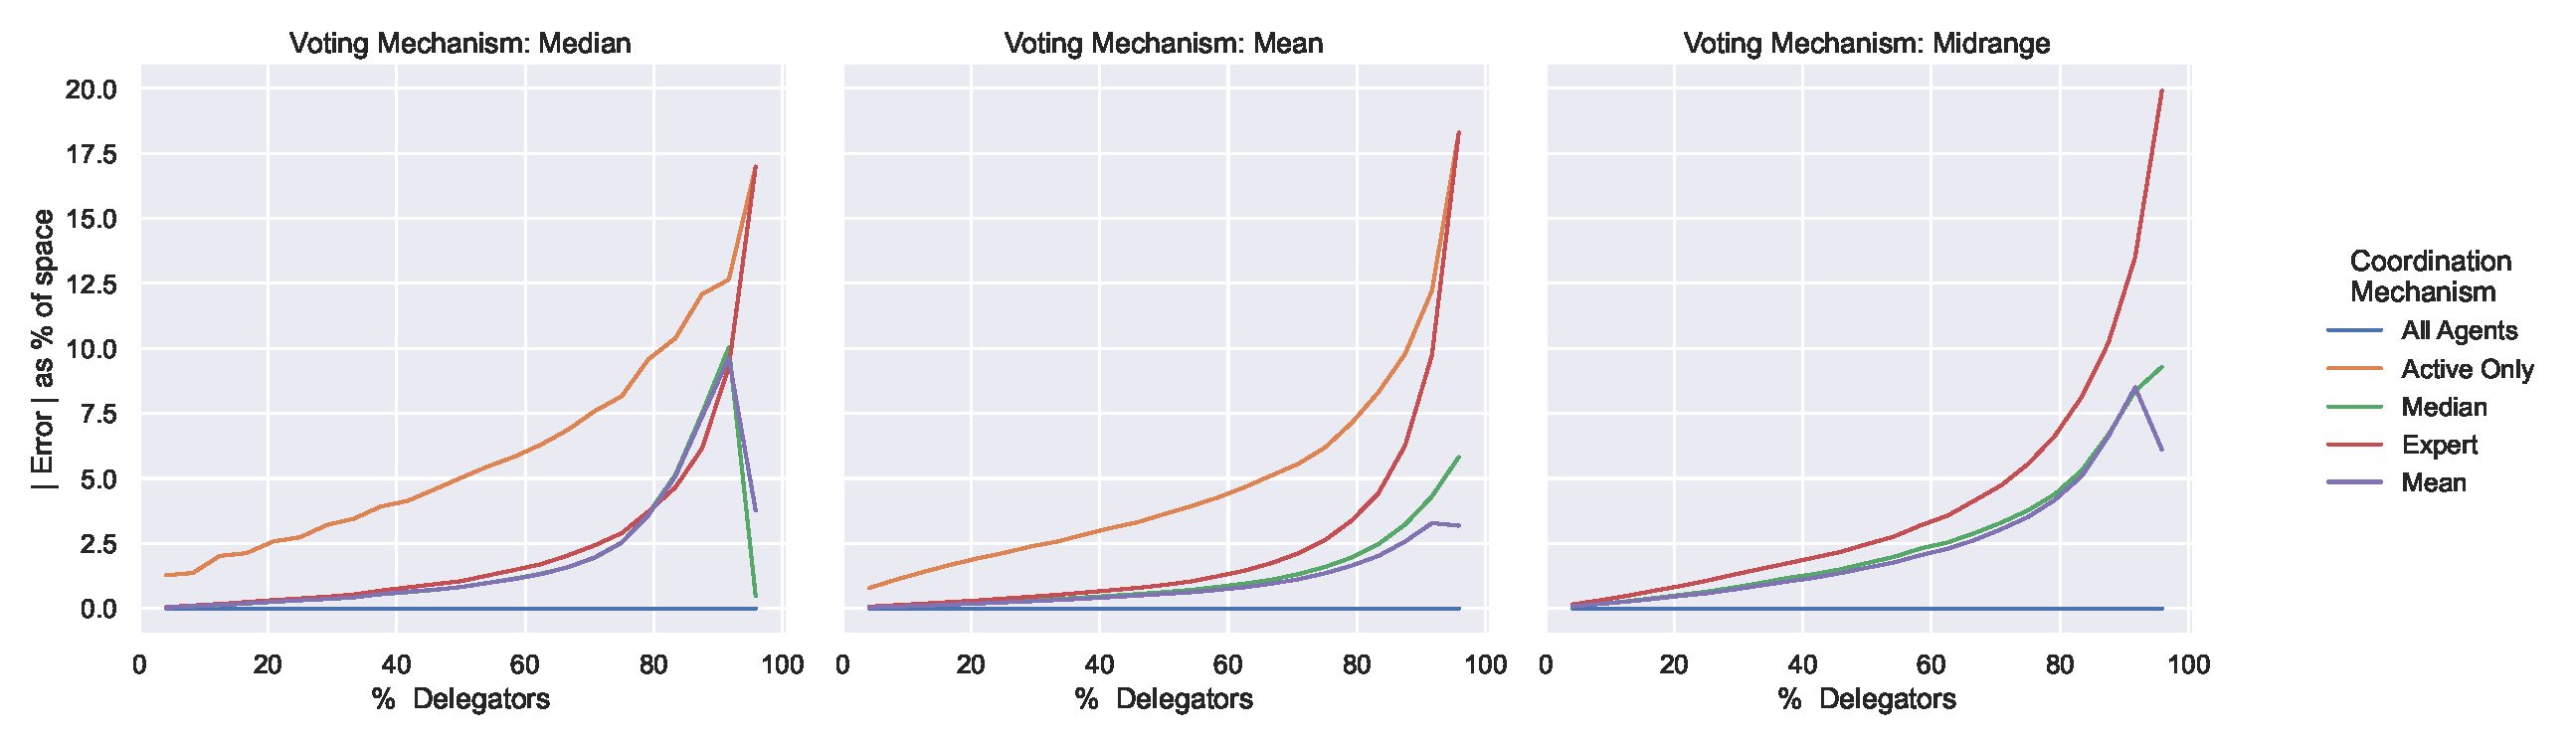
\includegraphics[scale=0.55]
        {content/chapter2/figures/vm_col_cm_hue_error_as_percent_of_space_abs_mean}
        \caption{
            The absolute mean error as a percent of the preference space by
            coordination mechanism per voting mechanism.
            `Error as a percent of the preference space' means the error divided by
            the total size of the preference space.
            Note All Agents represents when all agents are voting, meaning no proxy
            voting is used and all agents are present.
            Similarly, Active Only represents when proxy voting is not used and not
            all agents are present, and when proxies lose their constituents.
            The results are averaged over 1024 total runs.
            There are 24 total agents.
        }
        \label{fig:vm-col-cm-hue-error-as-percent-of-space-abs-mean}
    \end{figure}
\end{landscape}

\autoref{fig:different-weight-comparison}~shows there is an immediate difference from
when all agents have the same weight.
This is because, due to the weight, there is a shift towards the proxies' preferences
instead of the inactive voters'.
% 04/13: \vicki{which graphs are you referring to?  due to what?  unclear.}
% MDH: The referred-to graphs are specified in the previous sentence.
% I've re-referenced it here for clarification.
% The explanation for the error is in the next sentence.
Depending on the situation, this may be desirable.
Since the inactive agents are not participating they may not have as much information
and so their preference may not be as `up-to-date' as those who are actively
participating.
In situations where new information is constantly being introduced, such penalties
could be very valuable to ensure the most current information is being used.

Notably, the Median voting mechanism suddenly takes a sharp dip and produces a result
closer to all agents voting when using different weights than when using the same
weight.
This is strange since it is completely different compared to how any other
combination, or even the same combinations with less inactive voters, works.
With some inspection, one can find this dip is due to active voters having a
significantly larger influence compared to inactive voters.
With this setup, an active voter is worth 5 times the amount of weight than an
inactive voter.
Therefore, when an active voter's weight is added to the sum it is more able to push
the sum over the half-way mark, thereby making that active voter's preference the
median.
This is also why we see the most extreme dip with using the Median voting mechanism
with Median coordination mechanism: the proxy is able to reach the median both when
coordinating and when voting, thereby making the proxy and its constituents' vote be the
proxy's preference.
This makes the system less volatile, since votes are less likely to be an inactive
voter's, and so we don't see the large spike in error when a large percent of agents
are delegating.

Additionally, from~\autoref{fig:different-weight-comparison}, we see both the Median
and Mean voting mechanisms quickly increase
% 4/26/2023: \vicki{quickly increase in error? explain.  This is interesting as more
% delegators slows the affect. Better if x axis goes to 100\% as the other tables do.}
in difference before beginning to level out.
This is again due to the difference in weight between the active and inactive voters.
When both types of voters have the same weight, the coordination mechanisms help
ensure the loss of preference from the agent going inactive is minimal.
However, when they have different weights, in particular when the weight of the
inactive voters is substantially less than that of the actives, the results are more
akin to when the voter doesn't vote.

The Midrange voting mechanism, however, does not increase as quickly and does not
achieve as much of a difference.
Midrange, or $L_{\infty}$, takes the highest and lowest voting and averages the two.
This means it ignores weight, which is likely why the change in weights does not
affect it as much.
Any difference in the outcome, then, must come from the coordination mechanisms used
prior to the final vote being calculated with Midrange.

Notably, the Median mechanisms, both voting and coordination, yields the largest
change.
Mean is close behind, and Expert yields slightly less.
Since the Median voting mechanism has already been shown to be difficult to
manipulate~\cite{Moulin1980}, using both a Median voting and Median coordination
mechanism would likely be a good choice when choosing which mechanisms to use.

\begin{landscape}
    \begin{figure}[p]
        \centering
        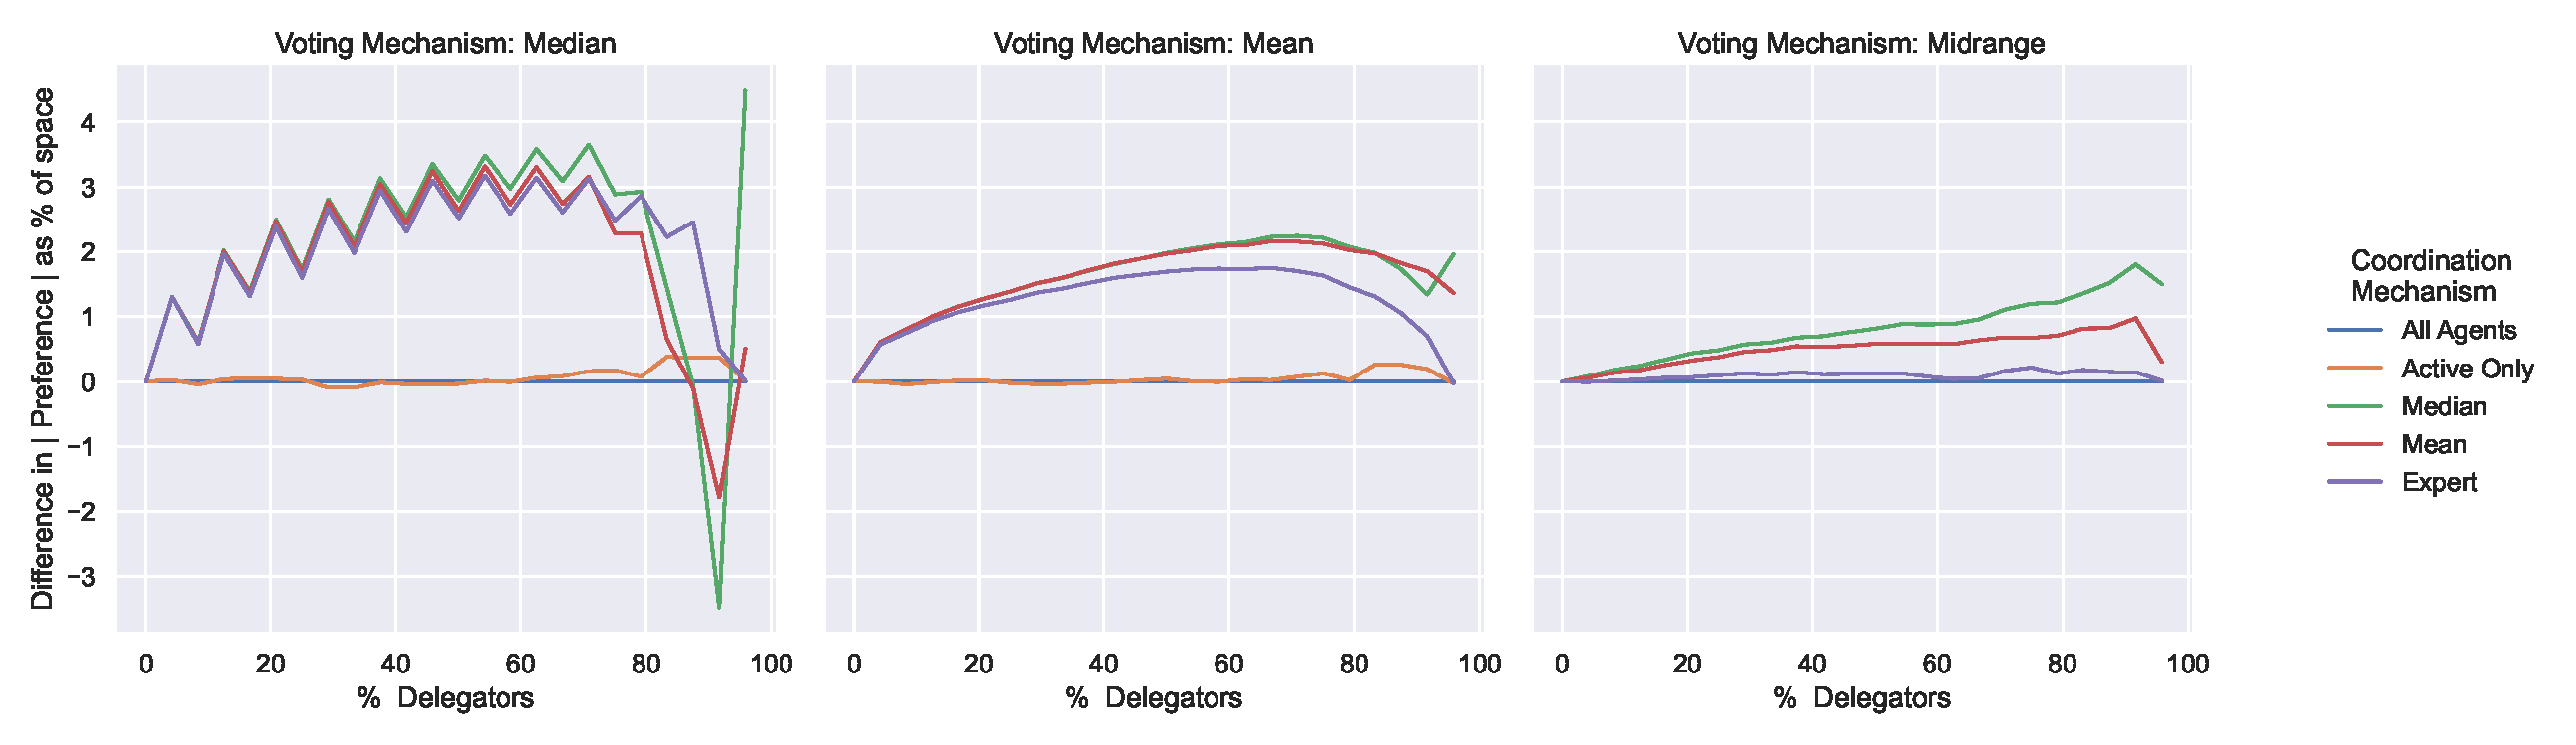
\includegraphics[scale=0.55]
        {content/chapter2/figures/different_weight/difference_abs_pref_percent_of_space}
        \caption{
            The difference between all agents having the same weight and inactive
            agents having only $\sfrac{1}{5}$ the weight as their proxies.
            The difference is in terms of distance as a percent of the preference
            space from all agents voting.
            `Distance as a percent of the preference space' means the absolute
            difference divided by the total size of the preference space.
            The results are averaged over 1024 total runs.
            There are 24 total agents.
        }
        \label{fig:different-weight-comparison}
    \end{figure}
\end{landscape}

\subsection{By Distribution}\label{subsec:results-distribution}
\autoref{fig:distribution-error-as-percent-of-space-abs-mean} shows
the absolute error as a percent of the preference space by coordination mechanism for
each voting mechanism and preference distribution.
\autoref{fig:distribution-different-scale-error-as-percent-of-space-abs-mean} shows
the same graphs, but with a different scale for each plot to more easily see the shape.
Additionally, each graph is zoomed in for readability
in~\autoref{apx:error-by-dist-zoomed}.

\vicki{Having three different versions of the same thing is painful when you are looking online, as you can't easily flip back and forth (or see them side by side). }

\begin{figure}[p]
    \centering
    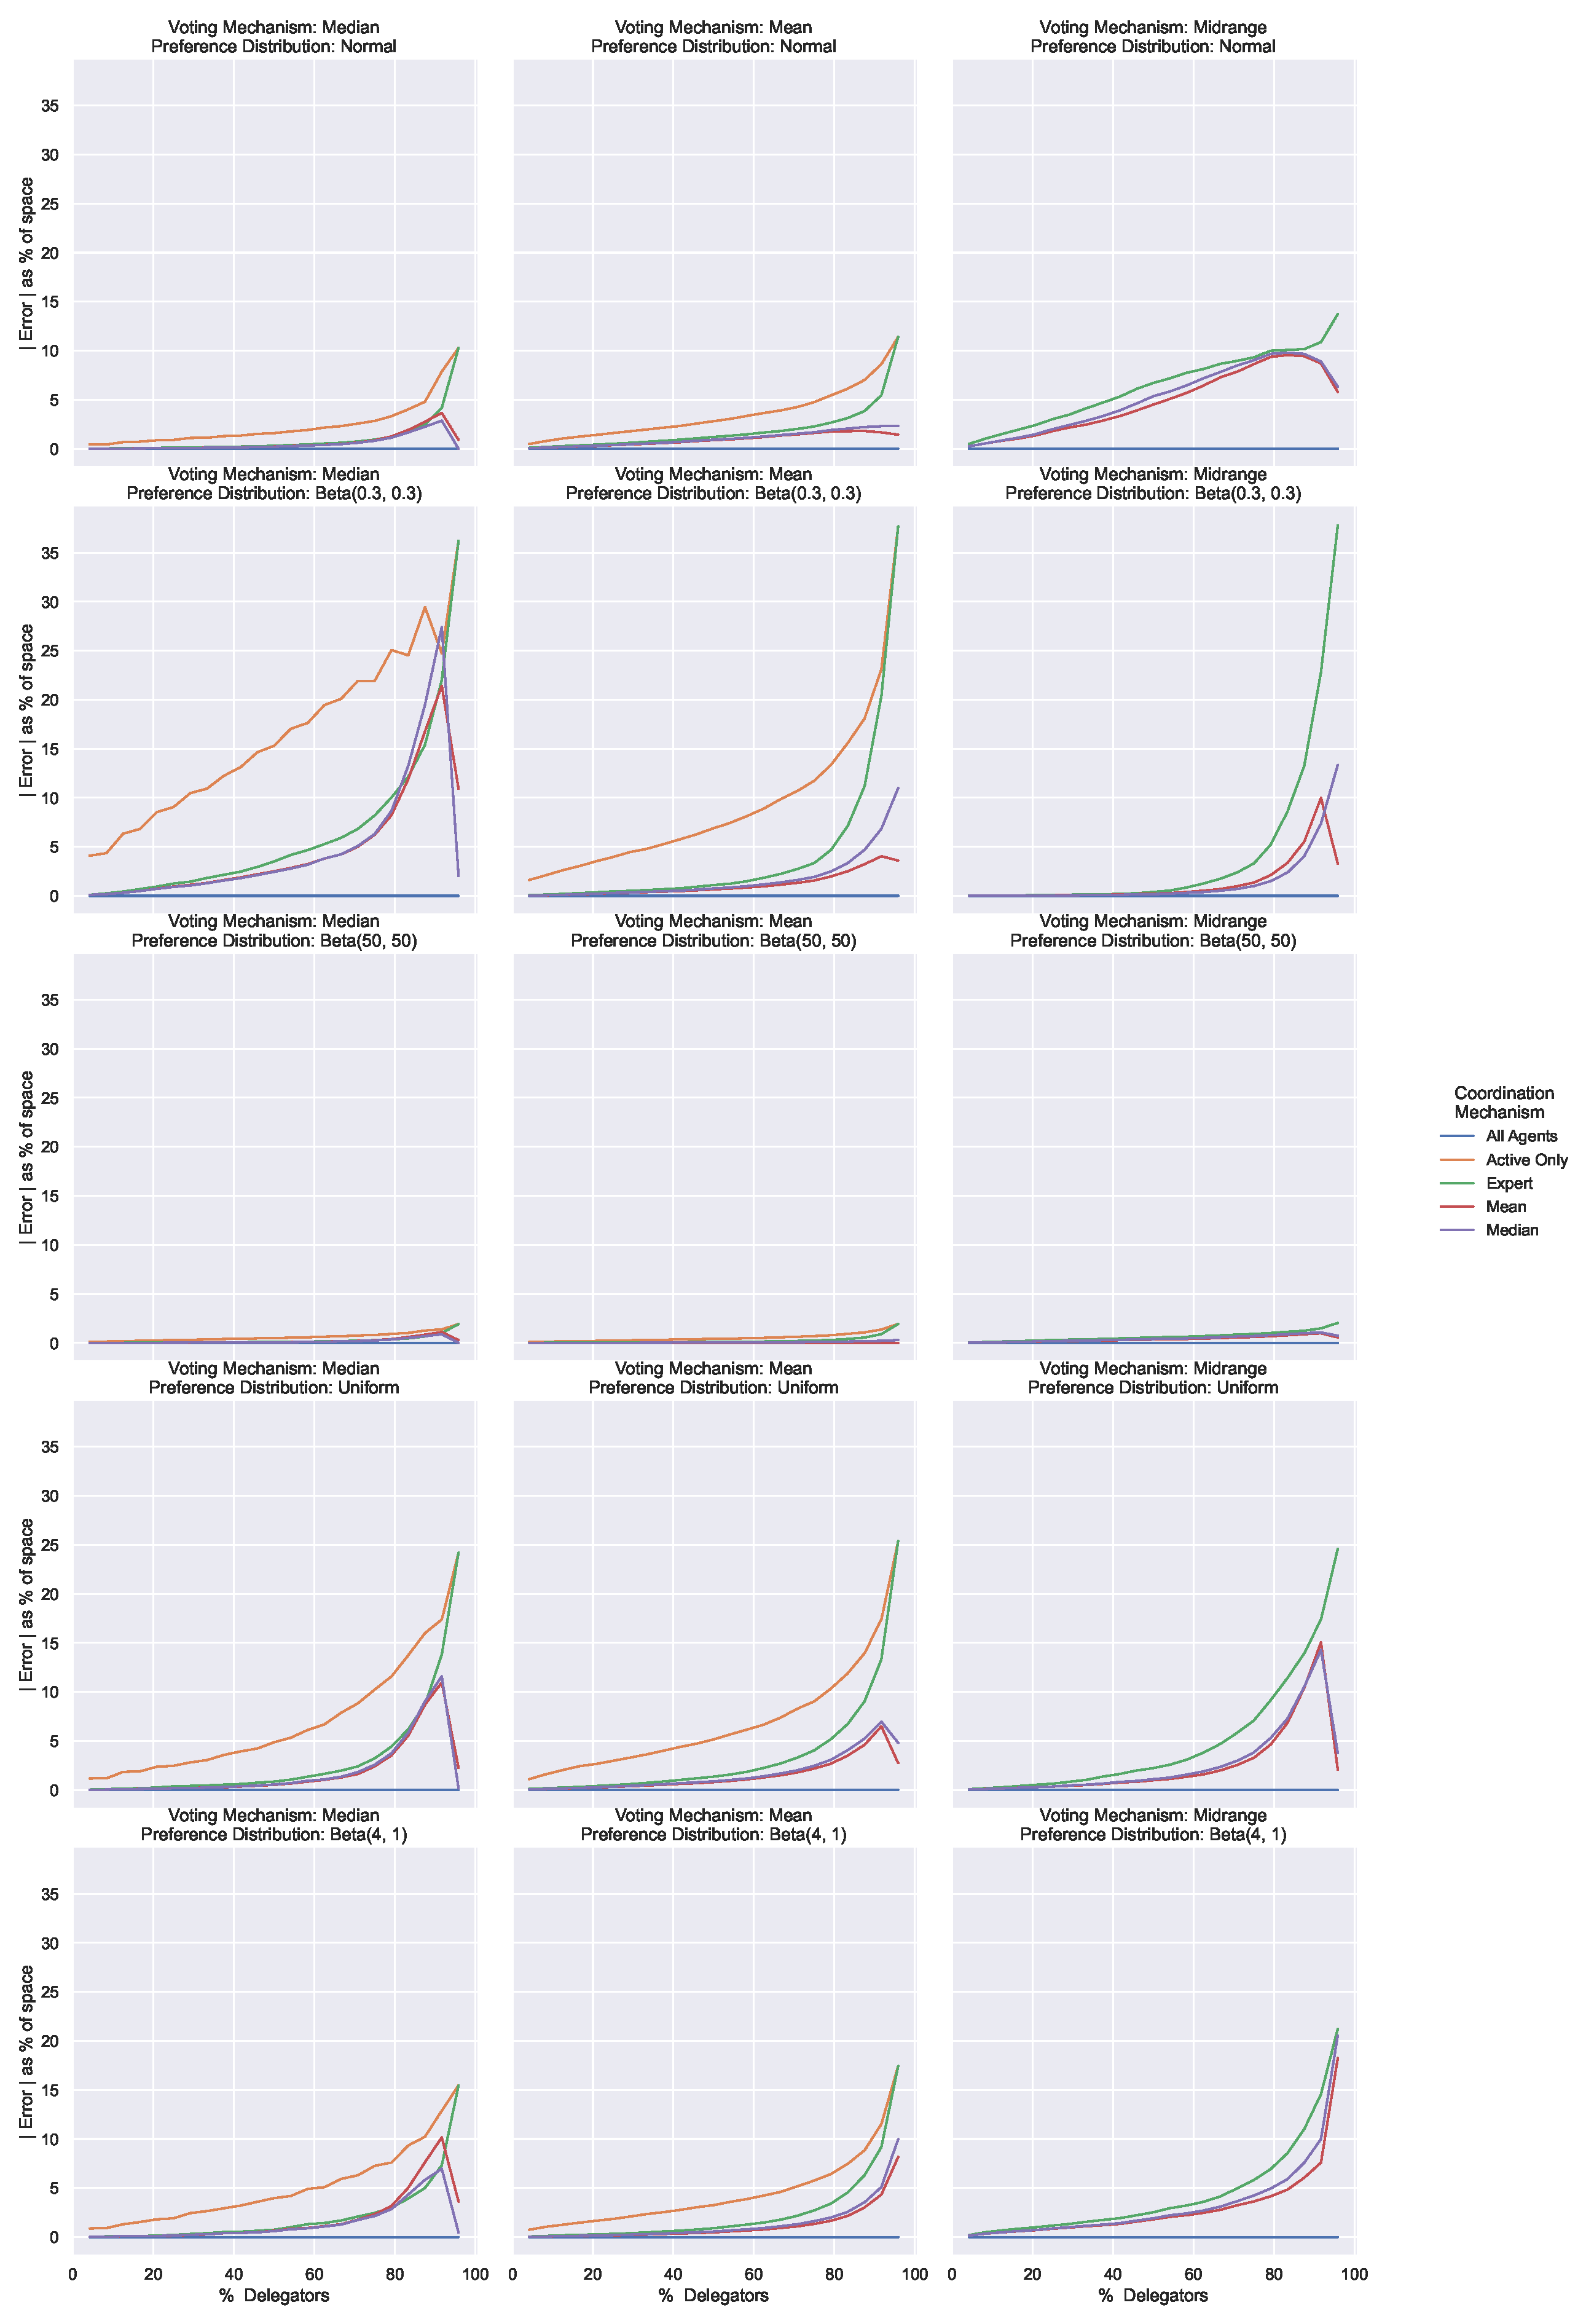
\includegraphics[scale=0.35]
    {content/chapter2/figures/distribution_error_as_percent_of_space_abs_mean}
    \caption{
        The absolute error as a percent of the preference space by coordination
        mechanism for each voting mechanism and preference distribution.
        The results are averaged over 1024 total runs.
        There are 24 total agents.
    }
    \label{fig:distribution-error-as-percent-of-space-abs-mean}
\end{figure}

Unsurprisingly, the tighter the probability density function (PDF) of a distribution,
the less error it has overall due to many votes being close to each other.
\betadistribution{50}{50} and Normal are two such distributions.
Nevertheless, these plots show the increase in error is consistent regardless of the
mechanisms or distributions used.
Mean and Median coordination mechanisms show a similar amount of error, while Expert
shows slightly more except when a large portion of the population is delegating and
when using the Midrange voting mechanism.
Interestingly, this seems to indicate again that it does not matter how you do proxy
voting so long as it is done.
Additionally, it should be noted the mechanisms perform well on most preference
distributions, including the asymmetrical distribution \betadistribution{4}{1}.

Unfortunately, while the error for other distributions is relatively similar,
\betadistribution{0.3}{0.3} yields considerably more error and starts accumulating
this error earlier when using the median voting mechanism.
\betadistribution{0.3}{0.3} represents a highly polarized topic, with its probability
density function having large spikes at either end of the preference space, making it
extremely important to ensure results are fair and accurate.
This would indicate that proxy voting, while it is still better than active-only
voting, does not work quite as well when agents have stronger, opposing opinions.

\vicki{  When you have a polarized topic, the answer chosen will always be a long distance from the preference.  For strong preferences, I'm guessing the mean or median is very volatile - changing dramatically from test to test, especially when the test size is small.  If the result changes wildly from test to test, we can hardly expect a different mechanism to change in the same wild way.  Is there a way we could verify this, say look at the standard deviation of resultant preference for the 1024 tests?   My guess is that for a normal distribution, the results are similar (for the same test, no proxy) from run to run, but that isn't true for other distributions. }

% 04/13:
% \vicki{
%     Why does this happen?
%     Is it because there are so few voters?
%     It would seem that two strong opinions shouldn't cause more error.
%     This needs to be explored as two opposing opinions is a common case.
% }
% MDH: See the following paragraphs where I explain why this could be.
% I've made a slight edit to specify this error really only occurs with the median
% voting mechanism.

For the median mechanism voting mechanism \vicki{specify the distribution}, the increase in error makes sense.
The median will most often be the preference of a specific agent, instead of some
value in between.
As such, the result will often be in one of the spikes in the PDF, since that is
where the majority of the agents' preferences will be, yielding higher error than when
using the Mean or Midrange voting mechanisms.
With the other voting mechanisms, the error is similar to other distributions using
the same mechanisms until the vast majority of the agents are inactive.
The increase in error is because as more agents go inactive there are fewer agents able
to serve as proxies, and so there may not be as desirable of a proxy to represent
each agent.

This finding is particularly important, as often the most polarizing topics are the
most important to individuals.
While it is still more beneficial to use proxy voting than not, in these polarized
cases, agents should make an extra effort to participate in-person to learn all they
can about the topic and ensure their voice is heard.
Those using proxy voting on split issues ought to be aware of this weakness and
implement some limitation to prevent inaccurate results.
These limitations could include requiring some percentage of the population, say
20--30\%, to be active.
Alternatively, if it becomes apparent that discussion is changing the opinions of the
active voters, which could be learned by occasionally polling the participants, it
may be wise to require voters to attend in person.
That way, those who have not been present to attend the deliberations can properly
participate.

\subsection{Preference Change}\label{subsec:results-shift}
\autoref{fig:abs-diff-from-preference-change-error-as-percent-of-space-abs-mean} shows
the difference in error between when proxies do have a preference change and when
they don't.
In this case, the proxies were able to shift their preferences by up to 10\% of the
total preference space, while delegators kept their original preference.
This represents the proxies changing their preference for an issue after deliberation.
\vicki{Explain how they change preference.  Are they influenced by the distribution?  I would guess if they were an outlier and changed preference, they would become more centrist.  Is this how you set it up?  If the changes are random, it doesn't seem realistic.}

Unsurprisingly, the amount of error increases as more agents become inactive.
However, the coordination mechanisms are much more tightly grouped than in other
scenarios.
We also see all voting mechanisms actually yield worse error than active-only
voting when using the Median and Mean coordination mechanisms.
This might be because delegators are selecting proxies who then shift a large amount,
leaving the delegator unsatisfied.

This potentially worse outcome highlights not only the importance of actively
participating in discussions, but also that when one needs to choose a proxy the
proxy must be someone who would act as the delegator who want them to act.

\begin{landscape}
    \begin{figure}[p]
        \centering
        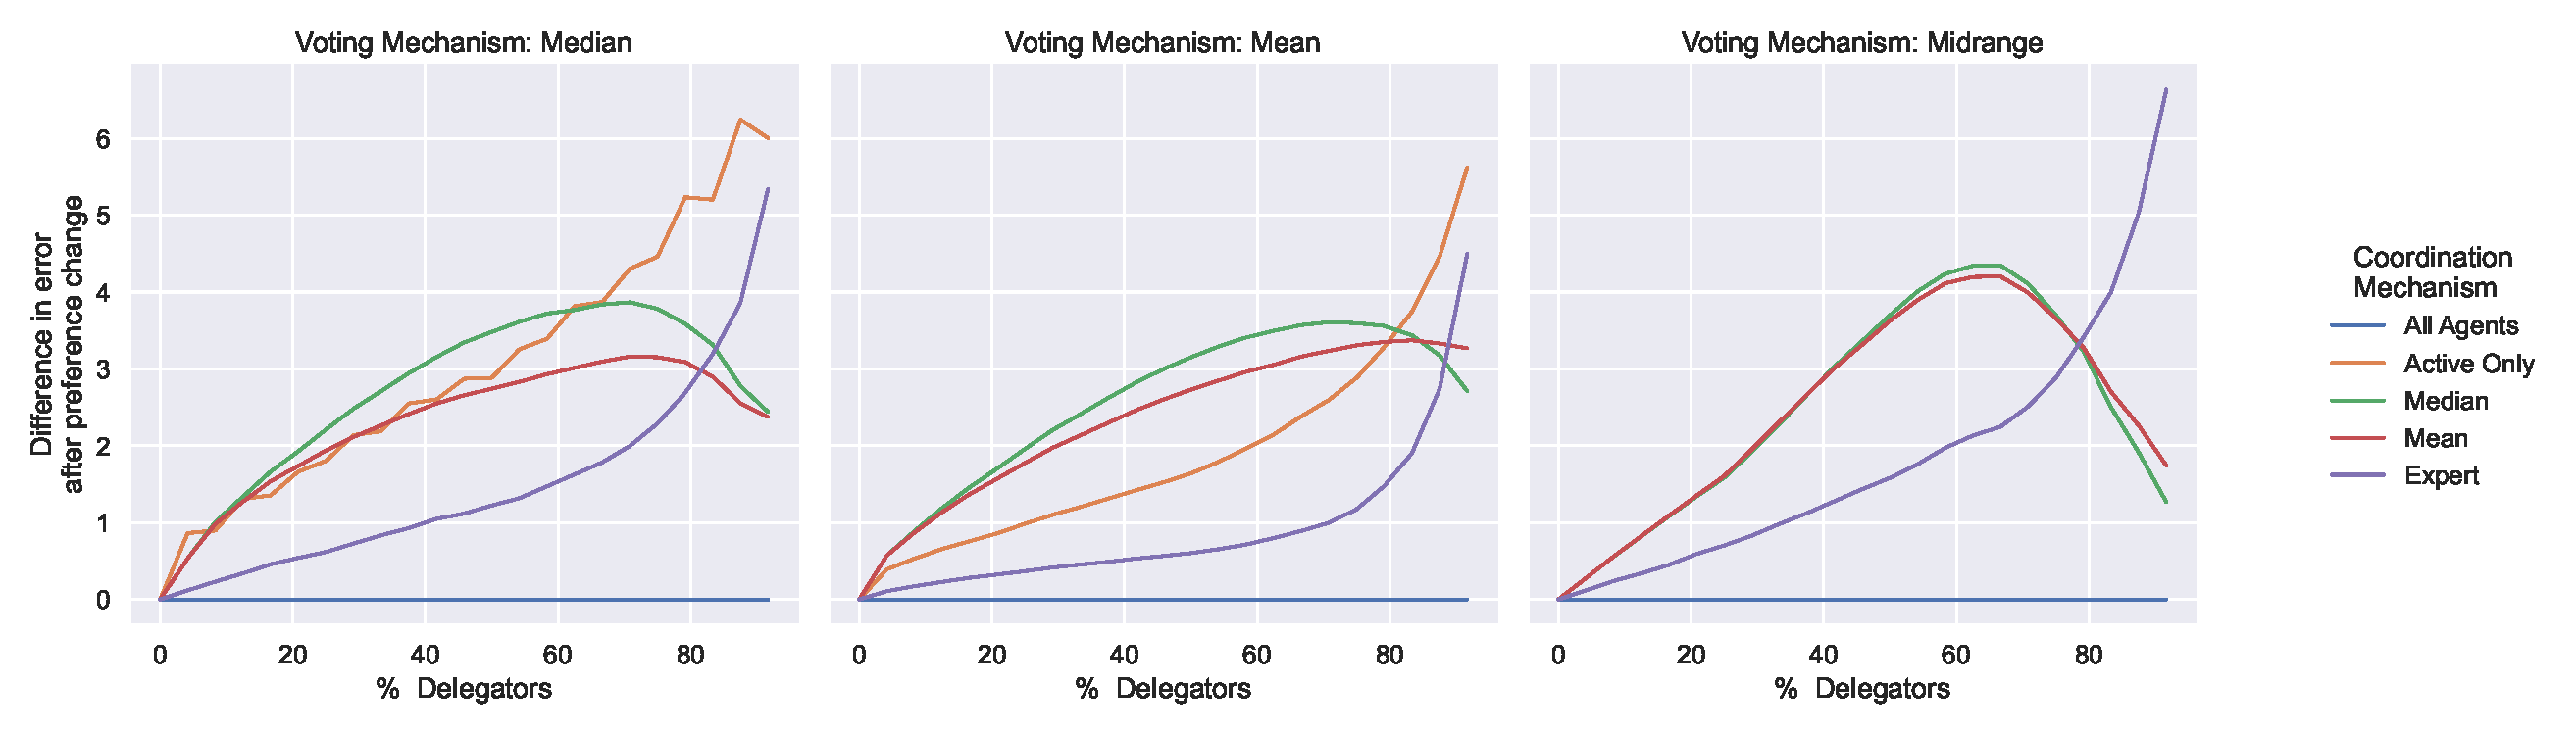
\includegraphics[scale=0.55]
        {content/chapter2/figures/abs_diff_from_preference_change_error_as_percent_of_space_abs_mean}
        \caption{
            The absolute difference in the error produced between without a
            preference change and with a preference change as a percent of space.
            The results are averaged over 1024 total runs.
            There are 24 total agents.
        }
        \label{fig:abs-diff-from-preference-change-error-as-percent-of-space-abs-mean}
    \end{figure}
\end{landscape}


    % Endmatter
% For BibTeX references: specify a .bib file and a style.
% The style used here is for IEEE transactions formatting:
\references{references/IEEEabrv,references/research}{IEEEtran}

% %
%  Example Appendix pages.
%  Modified to use new usu-thesis-mk2 appendix facilities.
%
%  Time-stamp: "[appendix.tex] last modified by Scott Budge (scott) on
%  2021-06-28 (Monday, 28 June 2021) at 09:03:44 on goga.ece.usu.edu"
%
%  Info: $Id: appendix.tex 1183 2021-06-28 16:49:30Z scott $   USU
%  Revision: $Rev: 1183 $
% $LastChangedDate: 2021-06-28 10:49:30 -0600 (Mon, 28 Jun 2021) $
% $LastChangedBy: scott $
%
%
% For a single appendix, use \makeappendix, and place the 
% body of the appendix after it

%\makeappendix

% < single appendix body here >

% For multiple appendices, use \makeappendices, and create each appendix
% using \appendix{}
% For sub-appendices use \appendixsection{} and \appendixsubsection{}

\makeappendices
\appendix{Voting Distributions}\label{chap:voting-distributions}

\appendixsection{Percent inside Extents}
% TODO: Add description of table
This is placeholder text to ensure
\autoref{tab:distributions-percent-inside-extents} stays in the correct
location. % FIXME

% - Distribution of votes
%     - Uniform
%     - Gaussian
%     - Bimodal about center
%     - Skewed?

\begin{table}[htbp]
    % increase table row spacing, adjust to taste
    \renewcommand{\arraystretch}{1.3}

    \caption{List of distributions used by agents to vote.}
    \label{tab:distributions-percent-inside-extents}

    \centering
    \begin{tabular}{|c|c|c|}
        \hline
        Distribution      & Notation      & Percent inside Extents \\
        \hline
        Uniform           & \uniformdist  & 100\%                  \\
        \hline
        Normal (Gaussian) & \gaussiandist & 99.7\%                 \\
        \hline
        Beta              & \betadist     & 100\%                  \\
        \hline
    \end{tabular}
\end{table}

\appendixsection{Distributions used}
% TODO: Add graphs of distributions used
\begin{table}[htbp]
    % increase table row spacing, adjust to taste
    \renewcommand{\arraystretch}{1.3}

    \caption{List of distributions used by agents to vote.}
    \label{tab:distributions}

    \centering
    \begin{tabular}{|c|c|c|}
    \end{tabular}
\end{table}

\appendixsection{Voting Mechanism P-Values}
\autoref{fig:all-voting-mechanisms-p-values} illustrates the p-values for all voting
mechanisms, given the alternative is one population is lesser than the other.
An arrow pointing to another voting mechanism indicates the `from' mechanism beats
the `to' mechanism.

\begin{figure}[!t]
    \centering
    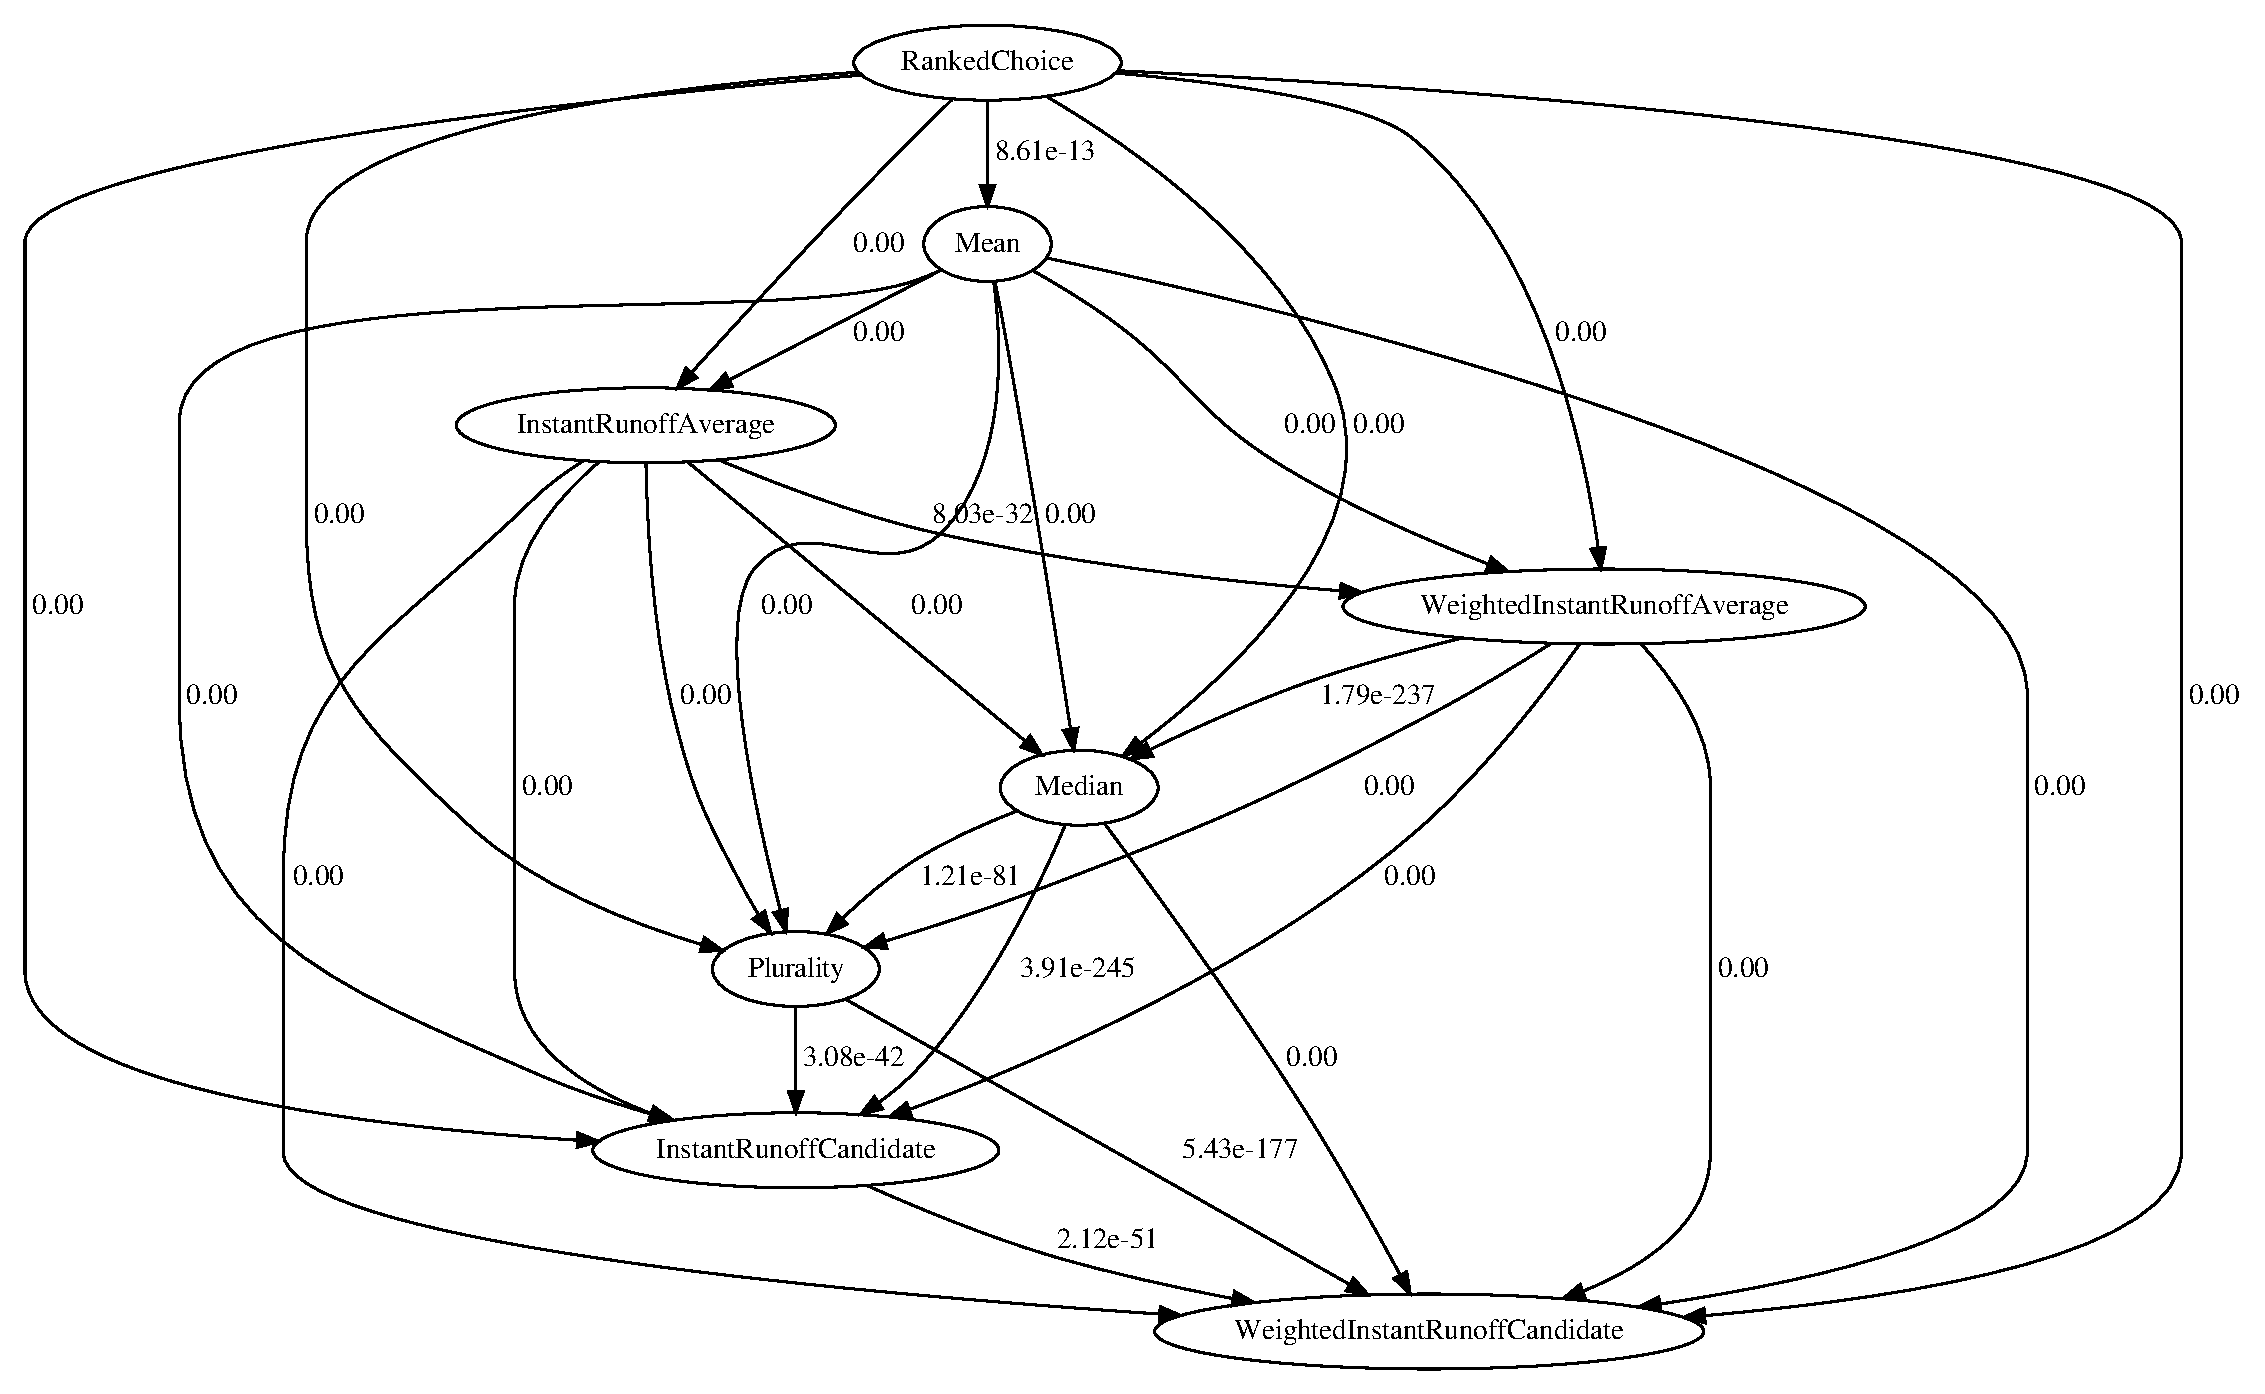
\includegraphics[
        angle=90,
        width=\textwidth,
        height=\dimexpr
        \textheight - 4 % Could also be .9\textheight
        \baselineskip,
        keepaspectratio]
    {./content/figures/voting_mechanisms/all-voting-mechanisms-p-values.gv}
    \caption{The p-values for all voting mechanisms, given the alternative is one
    population is lesser than the other.
    An arrow pointing to another voting mechanism indicates the `from' mechanism beats
    the `to' mechanism.}
    \label{fig:all-voting-mechanisms-p-values}
\end{figure}


\appendixsection{Distributions of Variables}
The distribution of variables for each voting mechanism is displayed as a
KDE graph in the figures of this section.

\begin{figure}[!t]
    \centering
    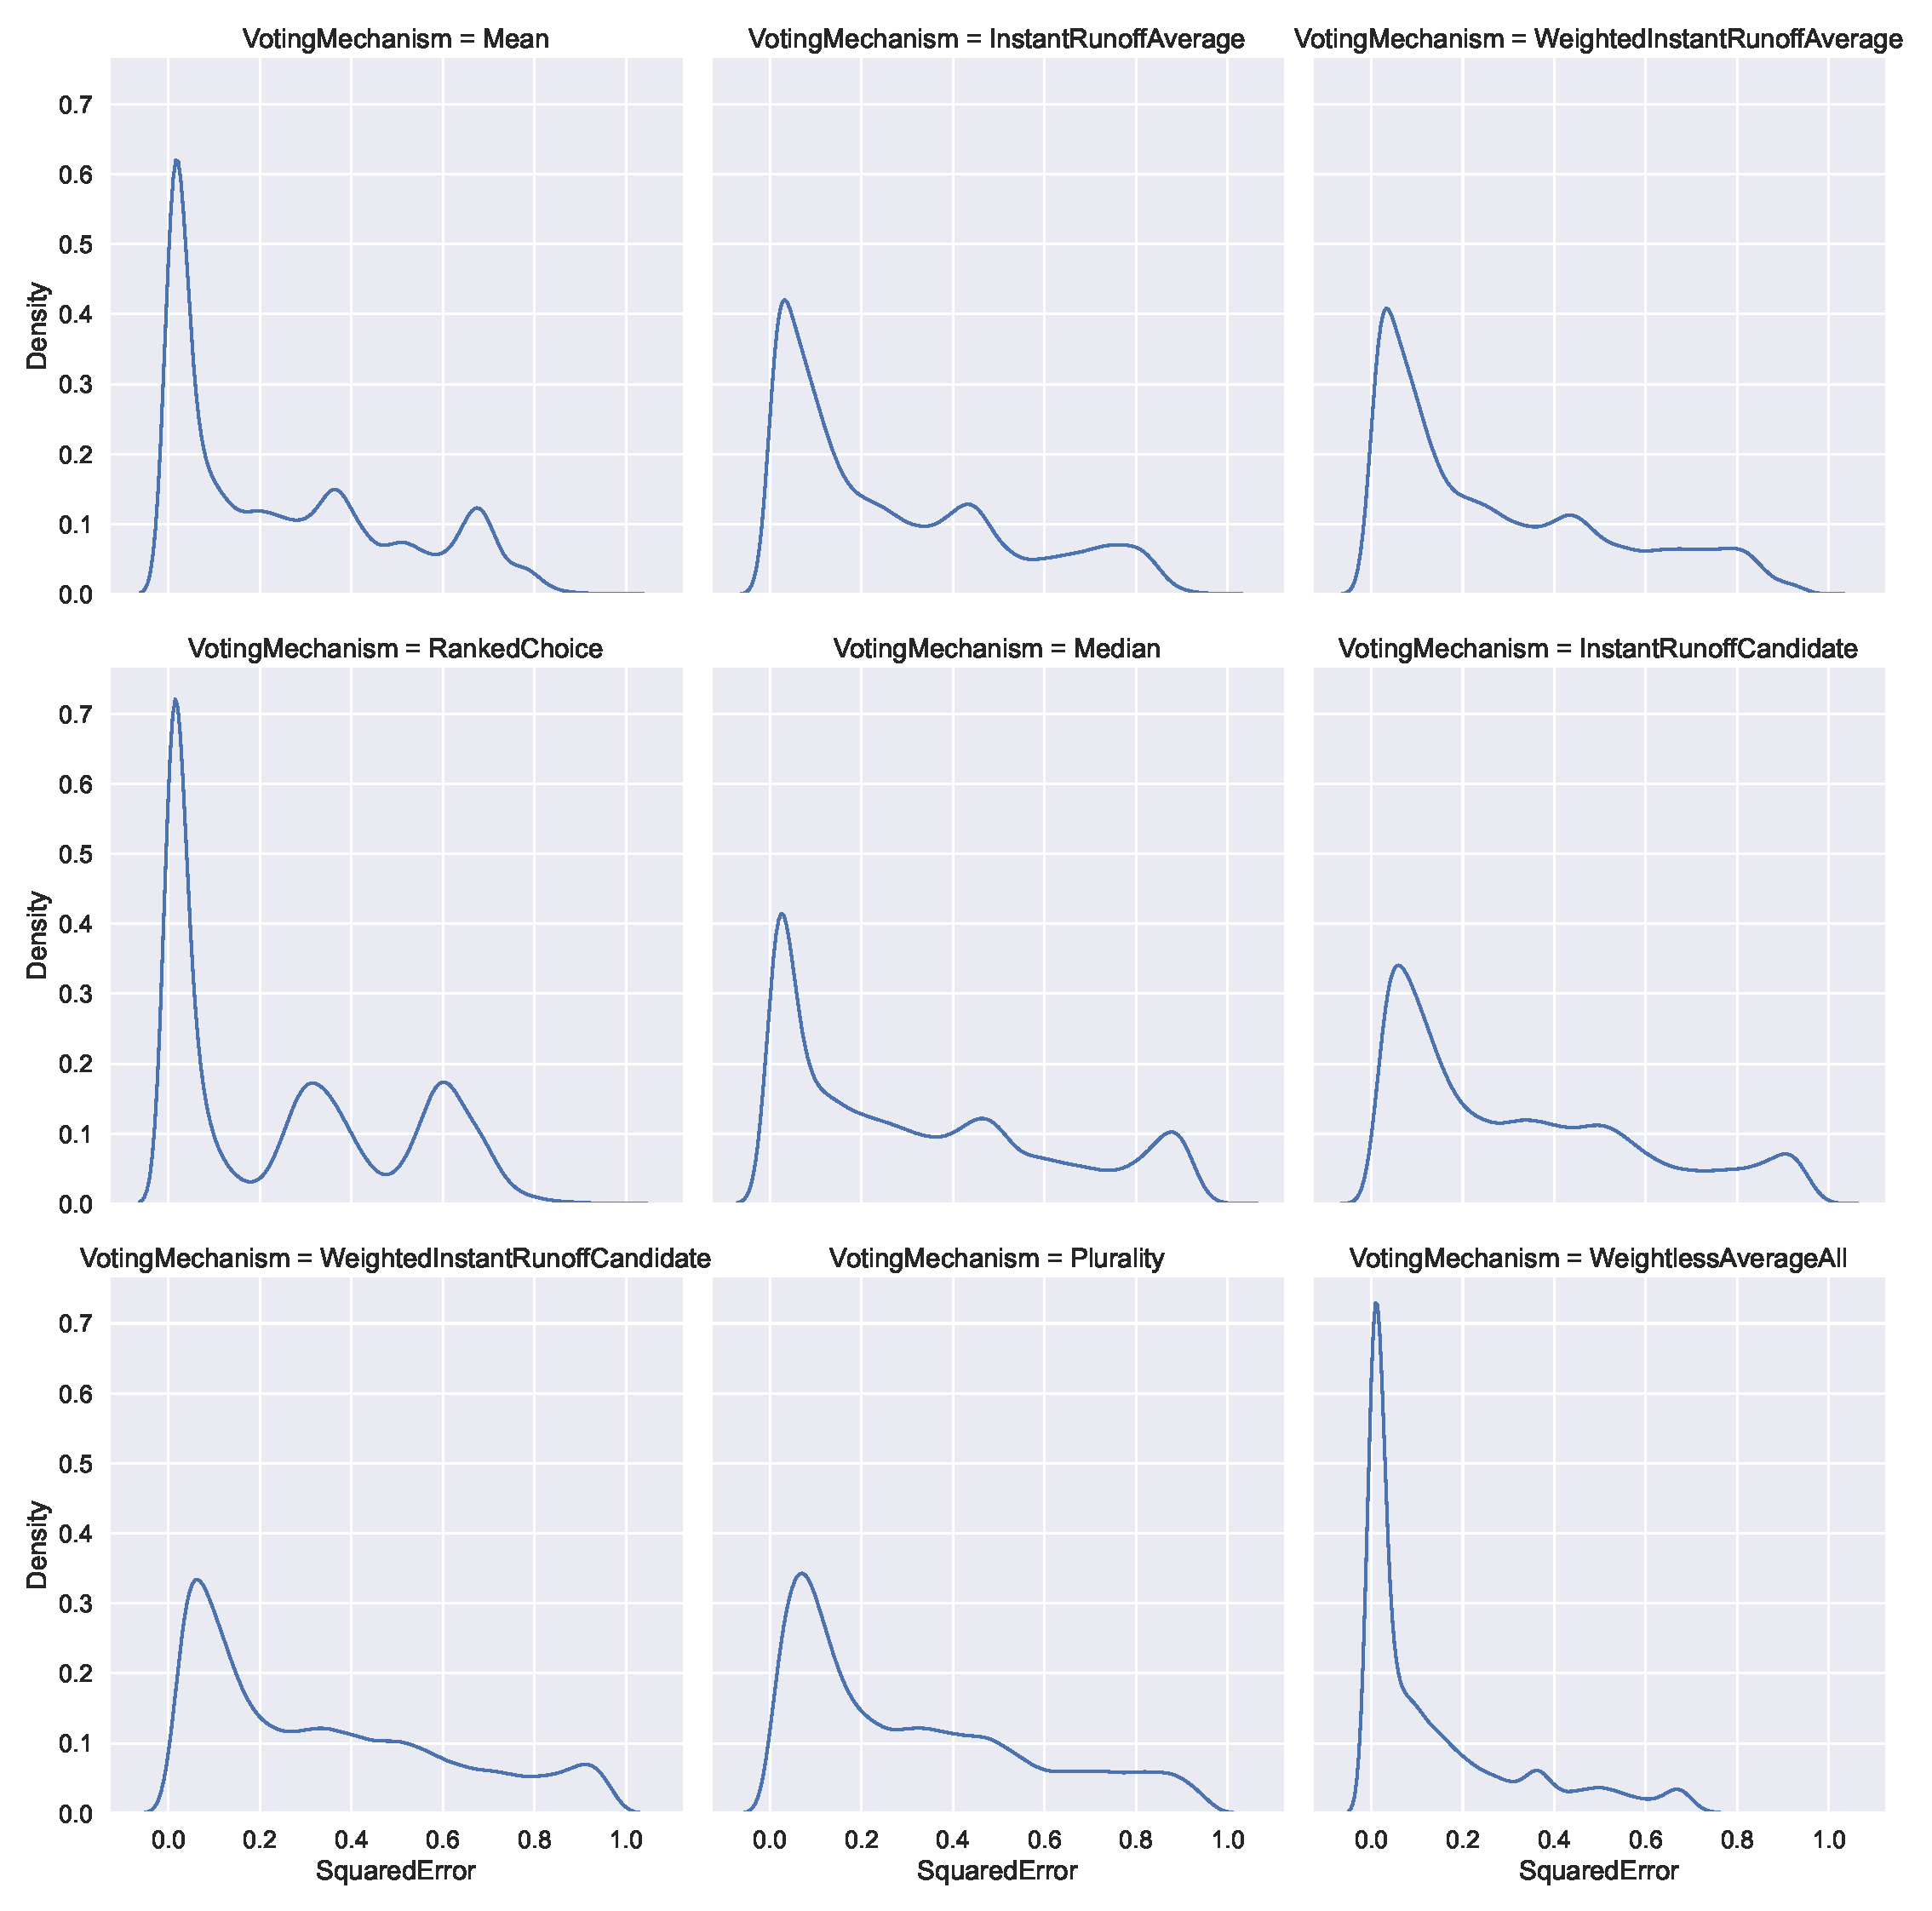
\includegraphics[
        width=\textwidth,
        height=\dimexpr
        \textheight - 2 % Could also be .9\textheight
        \baselineskip,
        keepaspectratio]
    {./content/figures/voting_mechanisms/voting_mechanisms_error_distribution}
    \caption{The distribution of squared error by voting mechanism.}
    \label{fig:voting_mechanisms_error_distribution}
\end{figure}

\begin{figure}[!t]
    \centering
    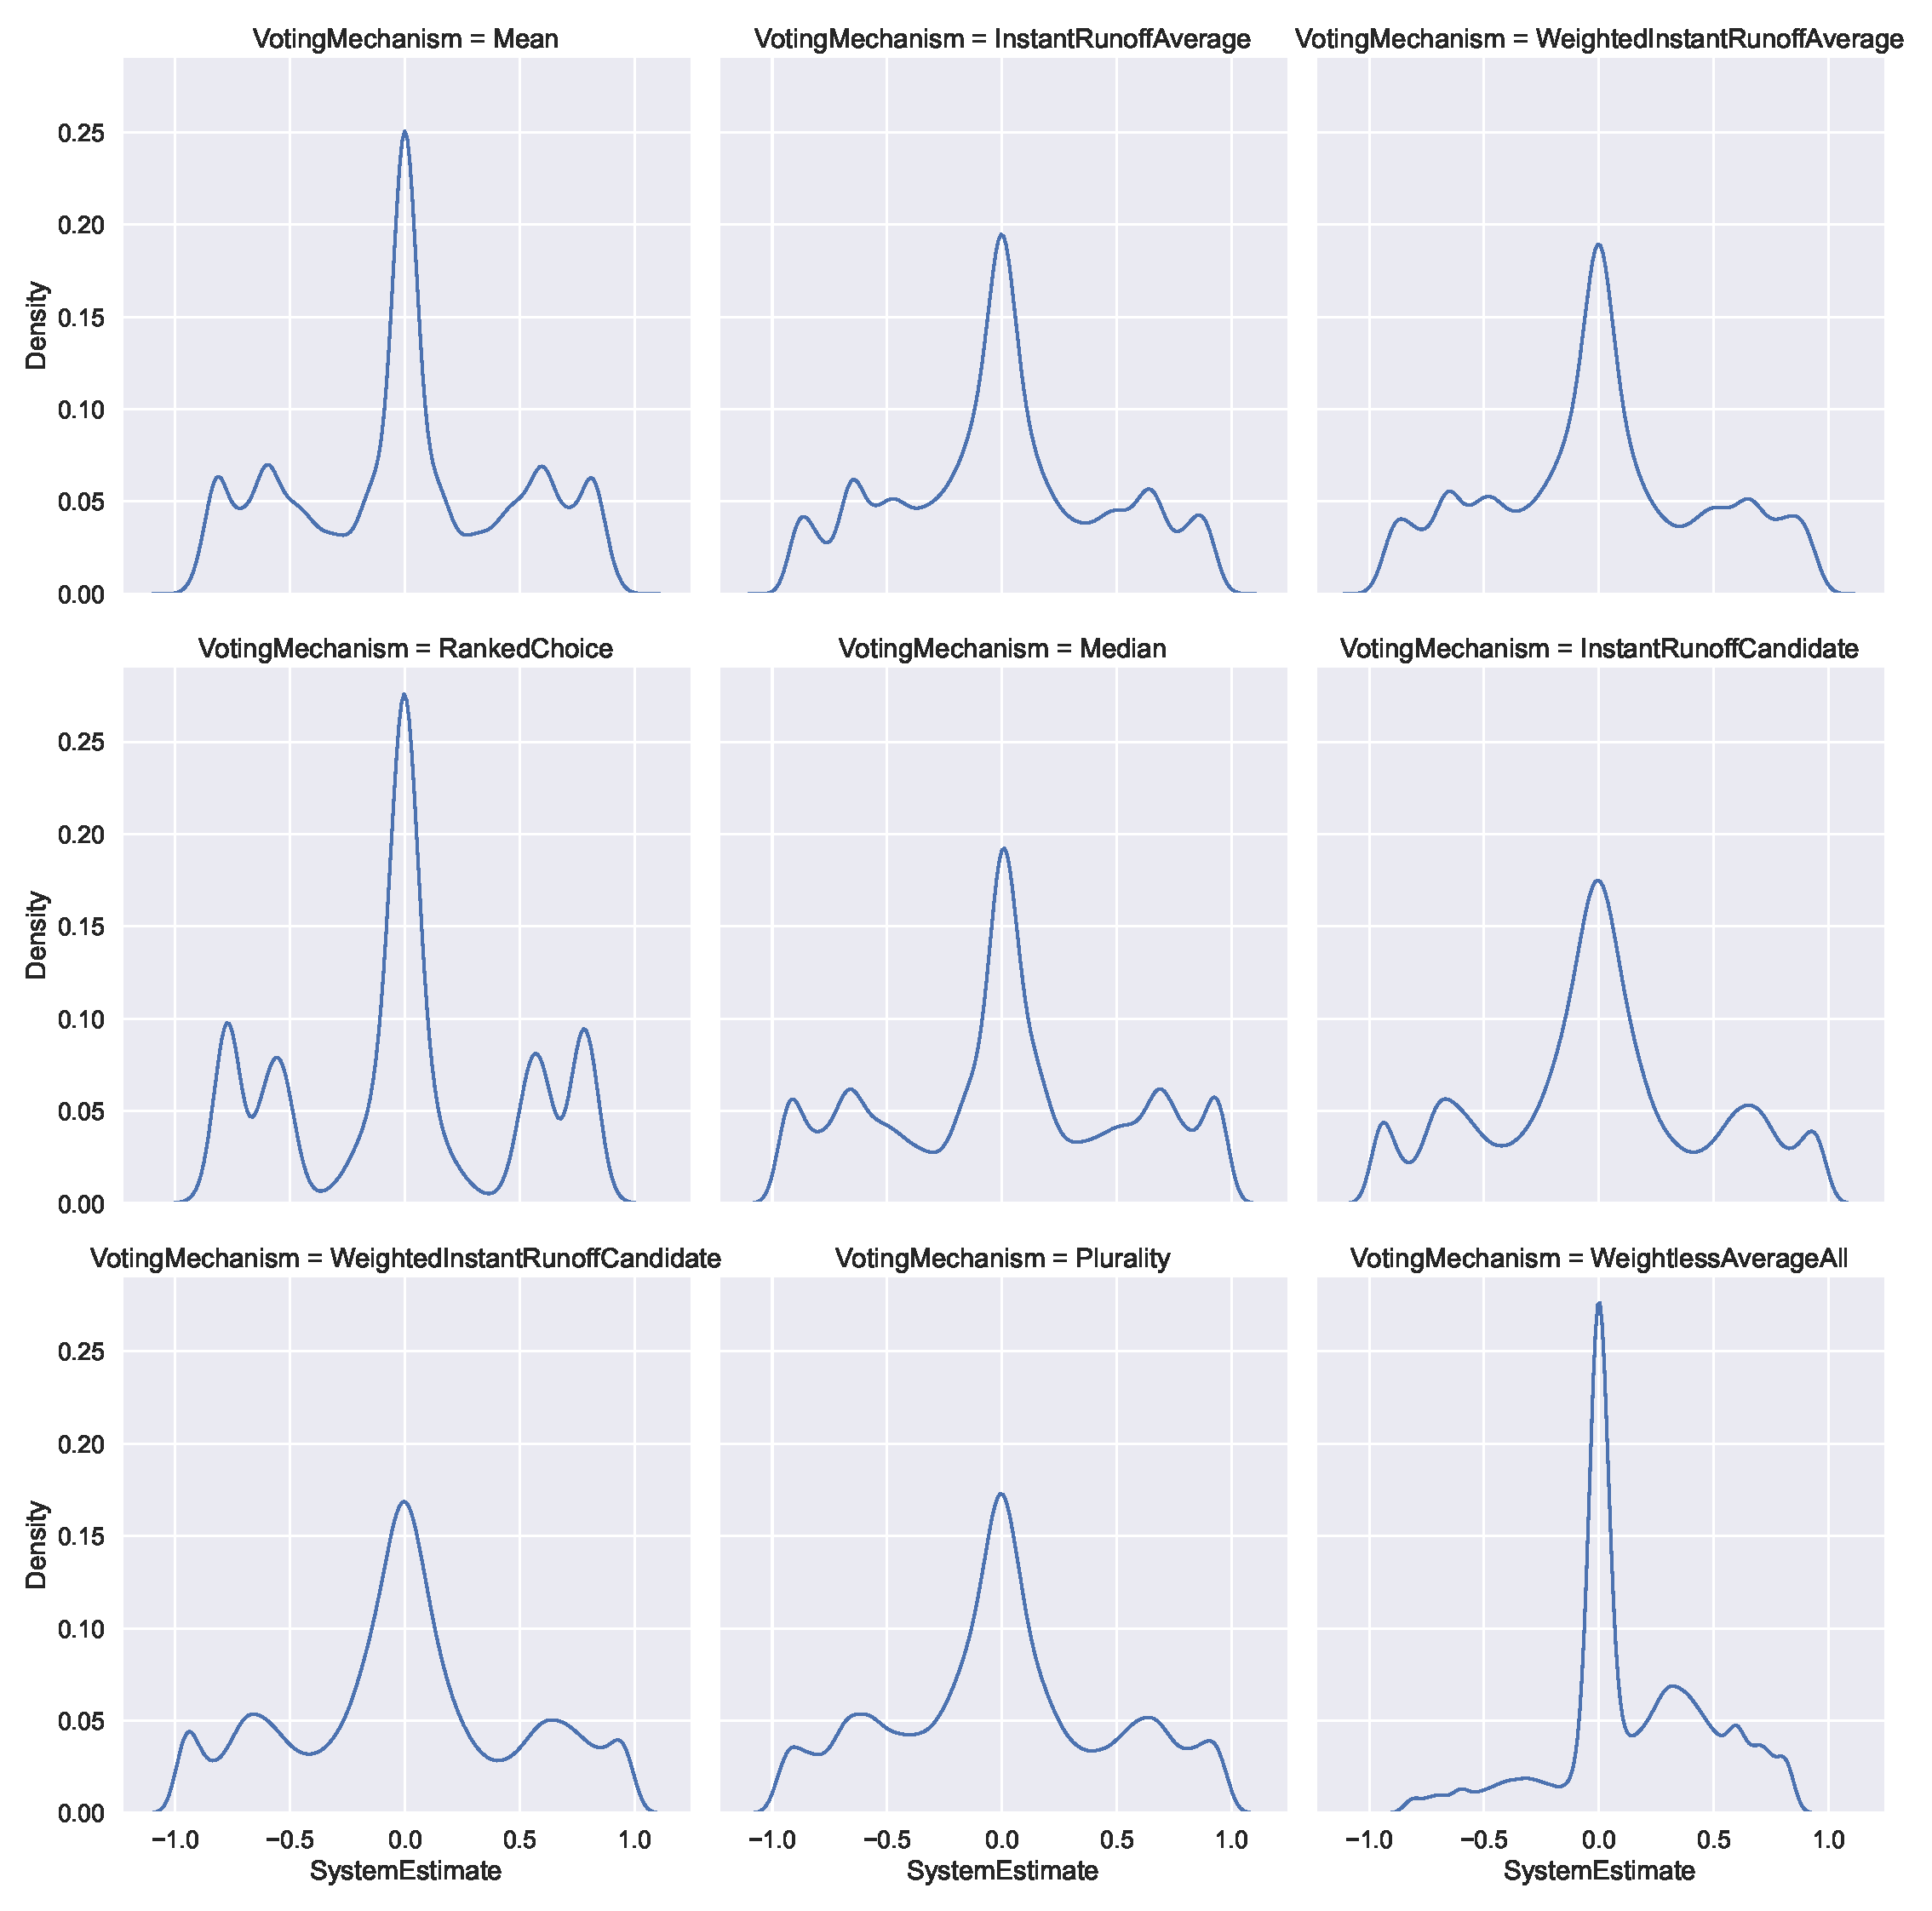
\includegraphics[
        width=\textwidth,
        height=\dimexpr
        \textheight - 2 % Could also be .9\textheight
        \baselineskip,
        keepaspectratio]
    {./content/figures/voting_mechanisms/voting_mechanisms_estimate_distribution}
    \caption{The distribution of system estimate by voting mechanism.}
    \label{fig:voting_mechanisms_estimate_distribution}
\end{figure}

\appendix{Visualizations}\label{chap:visualizations}
\begin{figure}[htbp]
    \centering
    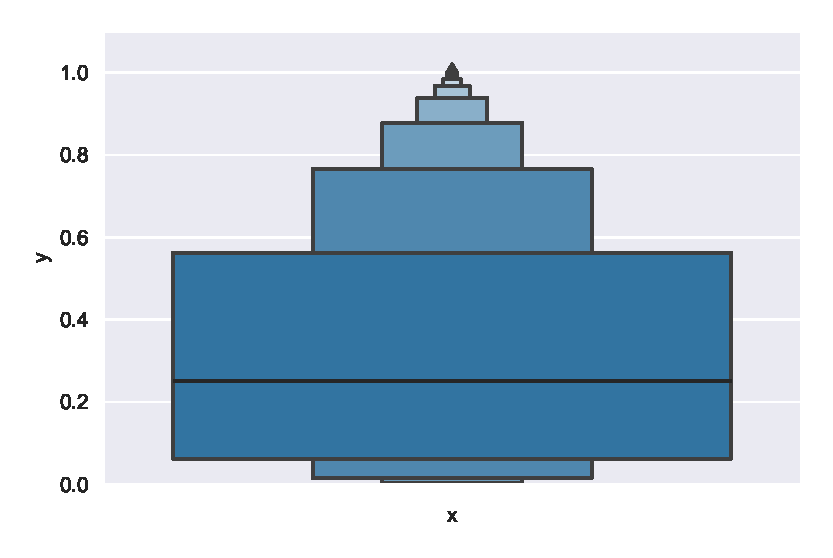
\includegraphics[scale=0.5]
    {./content/figures/expected_even_distribution_squared_error}
    \caption{Expected squared error distribution given a uniform distribution
    of estimates.}
    \label{fig:expected_even_distribution_squared_error}
\end{figure}

\begin{figure}[htbp]
    \centering
    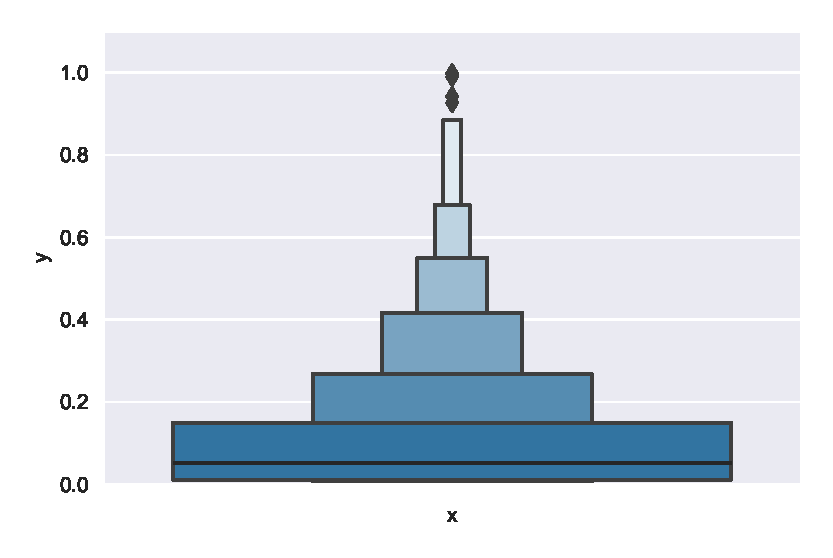
\includegraphics[scale=0.5]
    {./content/figures/expected_gaussian_distribution_squared_error}
    \caption{Expected squared error distribution given a gaussian distribution
    of estimates.}
    \label{fig:expected_gaussian_distribution_squared_error}
\end{figure}
 TODO Update

\end{document}
